\newif\ifshowsolutions
\showsolutionsfalse
\documentclass{article}
\usepackage{listings}
\usepackage{amsmath}
\usepackage{subfigure}
\usepackage{subfig}
\usepackage{bbm}
\usepackage{amsthm}
\usepackage{amsmath}
\usepackage{amssymb}
\usepackage{graphicx}
\usepackage{mdwlist}
\usepackage[colorlinks=true]{hyperref}
\usepackage{geometry}
\usepackage{titlesec}
\geometry{margin=1in}
\geometry{headheight=2in}
\geometry{top=2in}
\usepackage{palatino}
\usepackage{mathrsfs}
\usepackage{fancyhdr}
\usepackage{paralist}
\usepackage{todonotes}
\setlength{\marginparwidth}{2.15cm}
\usepackage{tikz}
\usetikzlibrary{positioning,shapes,backgrounds}
\usepackage{float} % Place figures where you ACTUALLY want it
\usepackage{comment} % a hack to toggle sections
\usepackage{ifthen}
\usepackage{mdframed}
\usepackage{verbatim}
\usepackage[strings]{underscore}
\usepackage{listings}
\usepackage{bbm}
\usepackage{bm}
\usepackage{algorithm}
\usepackage{algpseudocode}
\usepackage{mathtools}
\rhead{}
\lhead{}

\renewcommand{\baselinestretch}{1.15}

% Shortcuts for commonly used operators
\newcommand{\E}{\mathbb{E}}
\newcommand{\Var}{\operatorname{Var}}
\newcommand{\Cov}{\operatorname{Cov}}
\newcommand{\Bias}{\operatorname{Bias}}
\DeclareMathOperator{\argmin}{arg\,min}
\DeclareMathOperator{\argmax}{arg\,max}
\DeclareMathOperator{\arginf}{arg\,inf}
\DeclareMathOperator{\argsup}{arg\,sup}

% do not number subsection and below
\setcounter{secnumdepth}{1}

% custom format subsection
\titleformat*{\subsection}{\large\bfseries}

% set up the \question shortcut
\newcounter{question}[section]
\newenvironment{question}[1][]
  {\refstepcounter{question}\par\addvspace{1em}\textbf{Question~\Alph{question}\!
    \ifthenelse{\equal{#1}{}}{}{ [#1 points]}: }}
    {\par\vspace{\baselineskip}}

\newcounter{subquestion}[question]
\newenvironment{subquestion}[1][]
  {\refstepcounter{subquestion}\par\medskip\textbf{\roman{subquestion}.\!
    \ifthenelse{\equal{#1}{}}{}{ [#1 points]:}} }
  {\par\addvspace{\baselineskip}}

\titlespacing\section{0pt}{12pt plus 2pt minus 2pt}{0pt plus 2pt minus 2pt}
\titlespacing\subsection{0pt}{12pt plus 4pt minus 2pt}{0pt plus 2pt minus 2pt}
\titlespacing\subsubsection{0pt}{12pt plus 4pt minus 2pt}{0pt plus 2pt minus 2pt}


\newenvironment{hint}[1][]
  {\begin{em}\textbf{Hint: }}{\end{em}}


\chead{%
  {\vbox{%
      \vspace{2mm}
      \large
      Mass-friction\hfill
      Adjoint vs. Naive Gaussian \hfill \\[1pt]
      Rate-and-state friction\hfill
      January 10th, 2023
    }
  }
}
\newcommand{\la}{\left\langle}
\newcommand{\ra}{\right\rangle}
\newcommand{\indep}{\raisebox{0.05em}{\rotatebox[origin=c]{90}{$\models$}}}
\begin{document}
\pagestyle{fancy}
\section{Problem setup}
We consider a simple mass-block sliding on a horizontal surface driven by a spring moving at constant rate $V$, 
where the friction in between is rate-and-state dependent. 

\begin{figure}[H]
    \centering
    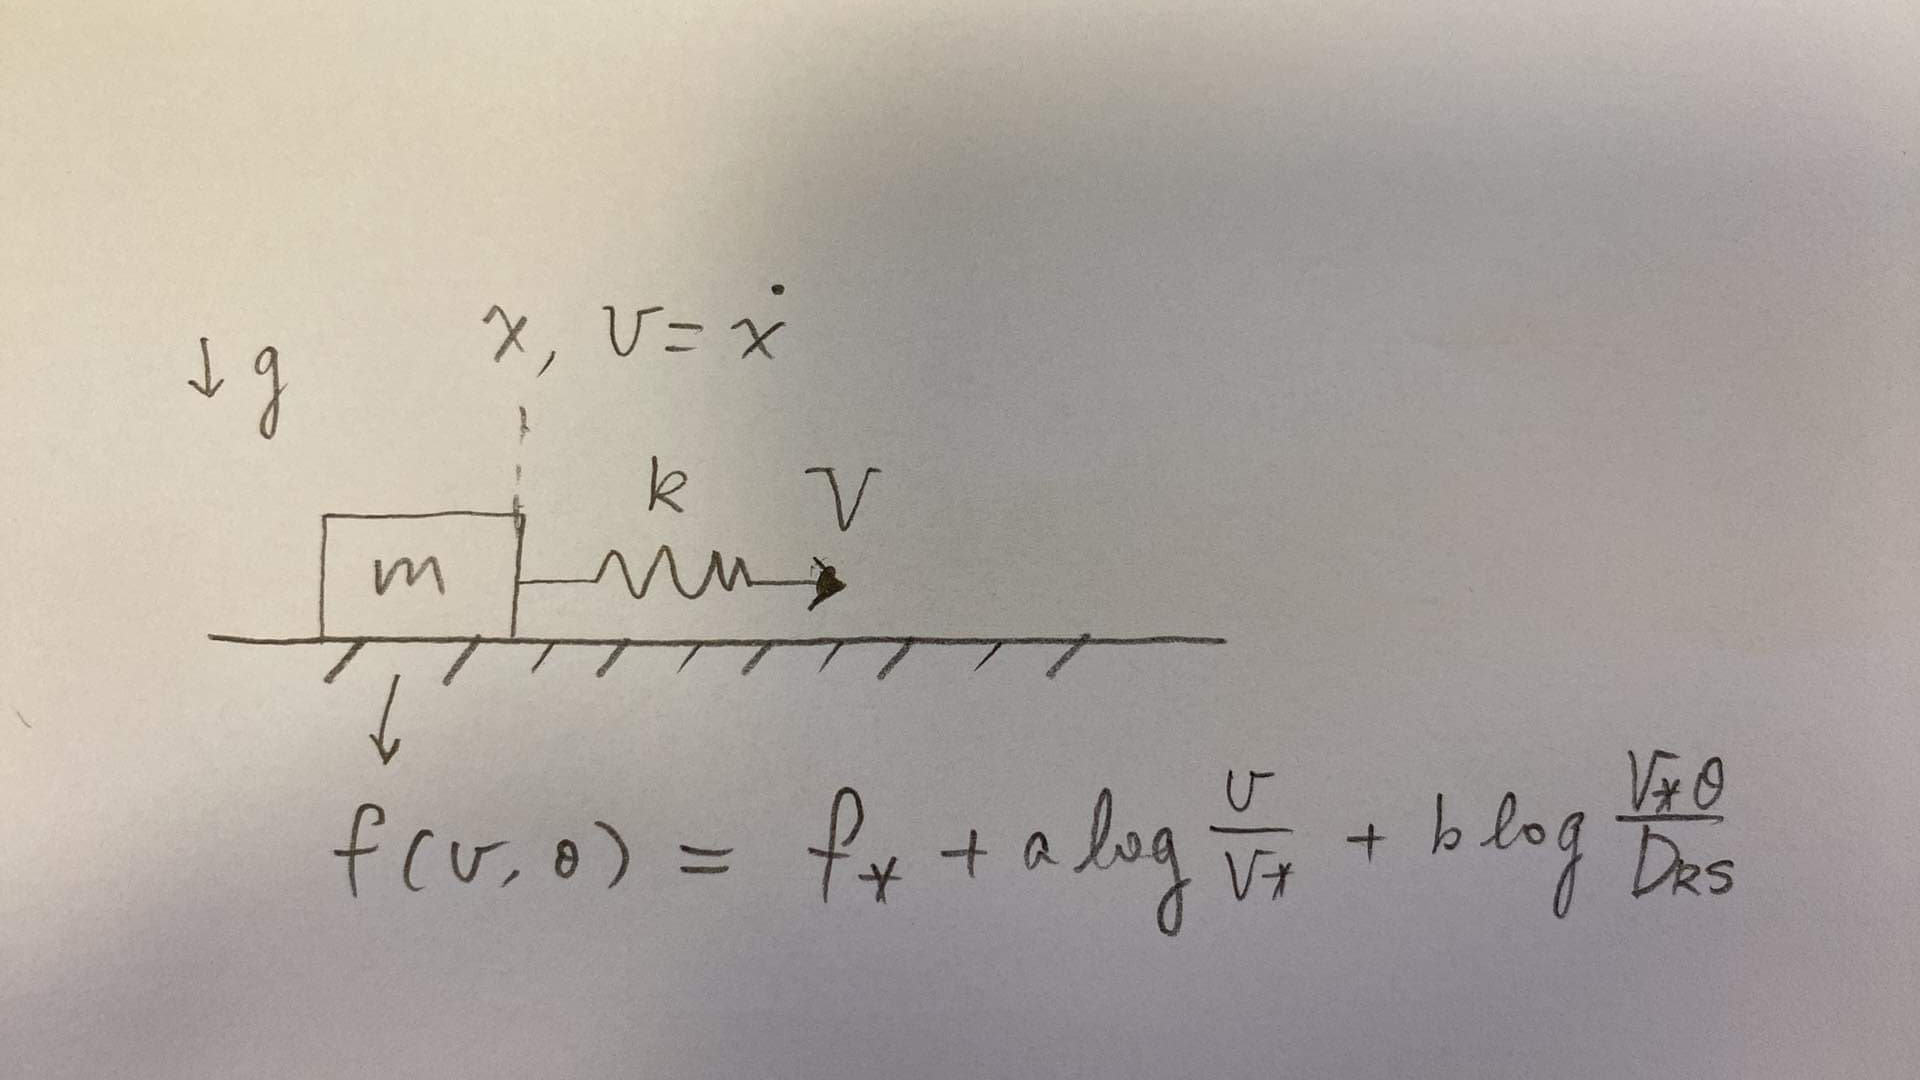
\includegraphics[width=0.8\textwidth]{shit1.png}
    \caption{Schematic figure of mass block sliding on a frictional surface}
    \label{fig:massBlockSliding}
\end{figure}

The parameters used: 
\begin{itemize}
    \item $k$: Stiffness of the spring
    \item $m$: Mass of the sliding block
    \item $V$: Constant speed at which the spring is being pulled
    \item $g$: Gravitational acceleration
    \item $x$: Position of the mass block
    \item $v$: Velocity of the mass block
    \item $\theta$: State variable
    \item $f(v=\dot{x}, \theta)$: Friction coefficient
    \item $t$: Time, within $[0, T]$
\end{itemize}

The equation of motion can be written as 
\begin{align}
    m\Ddot{x} + k(x - x_p) - mg\left[f_* + a\log(\dot{x}/V_*) + b \log(V_* \theta / D_{RS})\right] &= 0 \label{eq:motion}\\
    \dot{\theta} - (1 - \dot{x} \theta / D_{RS}) &= 0 \label{eq:evolutionAging}
\end{align}

The system has two generalized coordinates, 
\begin{align}
    \boldsymbol{q} &= [x, \theta]^T \label{eq:GenCoords}. 
\end{align}
We define inertia potential $E^{\text{in}}(\boldsymbol{q})$, 
elastic potential
$E(\boldsymbol{q})$ and 
dissipation potential $D(\boldsymbol{\dot{q}}, \boldsymbol{q})$ such that
\begin{align}
    \nabla_{\boldsymbol{q}} \left[E^{\text{in}}(\boldsymbol{q}) + E(\boldsymbol{q})\right] + \nabla_{\dot{\boldsymbol{q}}}D(\boldsymbol{\dot{q}}, \boldsymbol{q}_n) = 0 \label{eq:GenGradZero}
\end{align}
gives us (\ref{eq:motion}) and (\ref{eq:evolutionAging}).
\textbf{Note} that $\boldsymbol{q}_n$ and $\boldsymbol{q}_{n-1}$ are already known from previous time steps, 
and thus (\ref{eq:GenGradZero}) is not fully implicit, 
since the $D(\boldsymbol{\dot{q}}, \boldsymbol{q})$ has its second argument evaluated at the previous time step. 

Writing the potentials in terms of $\boldsymbol{q} = [x, \theta]^T$, 
if we define 

\begin{align}
    E^{\text{in}}(x, \theta) &= \frac{m}{2} \left(\frac{x - x_n}{\Delta t}\right)^2 \label{eq:Ein}\\
    E(x, \theta) &= \frac{k}{2}(x_p - x)^2 + \frac{\Delta t}{2} \left(\frac{\theta - \theta_n}{\Delta t}\right)^2 \label{eq:Eelastic}, 
\end{align}

\noindent then if we are able to find $D(\dot{x}, \dot{\theta}; x_n, \theta_n)$ such that 
\begin{align}
    \frac{\partial D}{\partial \dot{x}} &= -mg\left[f_* + a\log(\dot{x}/V_*) + b \log(V_* \theta_n / D_{RS})\right] \label{eq:proposeddDdx} \\
    \frac{\partial D}{\partial \dot{\theta}} &= - (1 - \dot{x} \theta_n / D_{RS}) \label{eq:proposeddDdTheta}, 
\end{align}
(\ref{eq:GenGradZero}) would be equivalent as am optimization problem:
\begin{align}
    \boldsymbol{q}_{n+1} &= \argmin_{\boldsymbol{q}} \left\{E^{\text{in}}(\boldsymbol{q}) + E(\boldsymbol{q}) + \Delta t D\left(\frac{\boldsymbol{q}-\boldsymbol{q}_n}{\Delta t}, \boldsymbol{q}_n\right)\right\} \label{eq:OptProb}. 
\end{align}
Actually now there is already an obviously problem, 
since $D$ is a relatively-smooth function of $\dot{x}, \dot{\theta}$, 
if you take a partial derivative of (\ref{eq:proposeddDdx}) w.r.t $\dot{\theta}$, 
and (\ref{eq:proposeddDdTheta}) w.r.t $\dot{x}$, 
you already can see that such a $D$ cannot exist unless $\theta_n$ is always $0$. 

But anyways, 
here's another argument, 
assuming such a $D(\dot{x}, \dot{\theta}; x_n, \theta_n)$ exists, 
starting from (\ref{eq:proposeddDdTheta}), 
we would have 
\begin{align}
    D(\dot{x}, \dot{\theta}) = -\dot{\theta} + \frac{\theta_n}{D_{RS}} \dot{x}\dot{\theta} + F_1(\dot{x}) \label{eq:DefF1}, 
\end{align}
plugging back into (\ref{eq:proposeddDdx}), 
we have a \textbf{problem of inconsistency}:
\begin{align}
    \frac{\theta_n}{D_{RS}} \dot{\theta} + F_1'(\dot{x}) &= \frac{\partial D}{\partial \dot{x}} = -mg\left[f_* + a\log(\dot{x}/V_*) + b \log(V_* \theta_n / D_{RS})\right] \label{eq:InconsProb}, 
\end{align}
where the right hand side only depends on $\dot{x}$, 
but the left hand side decisively has $\dot{\theta}$. 

This seems to mean that an additional term is needed in the rate-and-state friction formulation 
\begin{align*}
    f(\dot{x}, \theta) &= f_* + a\log(\dot{x}/V_*) + b\log(V_*\theta / D_{RS}). 
\end{align*}

% ------------- With slip law --------------
\section{Generalized gradient flow formulation with rate-and-state friction with slip evolution law}
For the evolution of state variable $\theta$ in rate-and-state friction, 
besides the aging law as stated in \ref{eq:evolutionAging}, 
there is another widely-used slip evolution law. 
And it is easier to find a Generalized Gradient Flow formulation that approximates that. 

With slip law, 
the equations of motion as in (\ref{eq:motion}) remains the same, 
which is 
\begin{align*}
    m\Ddot{x} + k(x - x_p) - mg\left[f_* + a\log(\dot{x}/V_*) + b \log(V_* \theta / D_{RS})\right] &= 0
\end{align*}
while (\ref{eq:evolutionAging}) changes into 
\begin{align}
    \dot{\theta} + \frac{\dot{x}\theta}{D_{RS}} \log\left(\frac{\dot{x}\theta}{D_{RS}}\right) &= 0 \label{eq:evolutionSlip}. 
\end{align}
If we define 
\begin{align}
    E(x, \theta) =& \frac{m}{2}\left(\frac{x-x_n}{\Delta t}\right)^2 + \frac{k}{2}(x_p-x)^2 + mg\frac{\Delta t}{2} \left(\frac{\theta-\theta_n}{\Delta t}\right)^2 \label{eq:ESlip}\\
    D(\dot{x}, \dot{\theta}) =& -mg\left[
    \left(f_*+b\log\frac{V_*\theta_n}{D_{RS}}-a\log V_*\right) \dot{x} 
    +a\dot{x}(\log \dot{x} - 1)
    + \dot{\theta} \frac{\dot{x}\theta_n}{D_{RS}}\left(\log \frac{\dot{x}\theta_n}{D_{RS}} - 1\right)\right] \label{eq:DSlip}, 
\end{align}
one would have 
\begin{align}
    \frac{\partial D}{\partial \dot{x}} &= -mg\left[f_* + a\log\left(\frac{\dot{x}}{V_*}\right) + b \log\left(\frac{V_* \theta}{D_{RS}}\right) \textcolor{red}{+ \frac{\dot{\theta}\theta_n}{D_{RS}}\log \left(\frac{\dot{x}\theta_n}{D_{RS}}\right)}\right]\label{eq:dDdxSlip} \\
    \frac{\partial D}{\partial \dot{\theta}} &= -mg\frac{\dot{x}\theta_n}{D_{RS}}\left[\log \left(\frac{\dot{x}\theta_n}{D_{RS}}\right)\textcolor{red}{-1}\right]
\end{align}

% Using Neural Network to find potentials
\newpage
\section{Using Neural network to find potentials for Rate and State friction}
\begin{comment}
\subsection{Taking $F_{fric}(x, \xi)=\frac{\partial W}{\partial x}(x, \xi)$}
Assuming the friction $F_{fric}$ at time $t$ given sliding history $x(t), t \in [0, t]$ is the solution of the following ODE system:
\begin{align}
    F_{fric}(x, \boldsymbol{\xi}) &= \frac{\partial W}{\partial x} \label{eq:potentialW}\\
    \frac{d D}{d \dot{\boldsymbol{\xi}}} + \frac{\partial W}{\partial \boldsymbol{\xi}} &= 0 \label{eq:potentialD}, 
\end{align}
where $W = W(x, \boldsymbol{\xi}), D = D(\dot{\boldsymbol{\xi}})$, 
$x$ is displacement, 
$\bm{\xi} \in \mathbb{R}^d$ is the state variable vector. 
Then the equilibrium equation in (\ref{eq:motion}):
\begin{align*}
    F^{inertia}(x) + F^{spring}(x) + F^{fric}(x, \bm{\xi}) = 0
\end{align*}
can be written as 
\begin{align}
    \frac{\partial E^{inertia}}{\partial x}(x) + \frac{\partial E^{spring}}{\partial x}(x) + \frac{\partial W}{\partial x}(x, \bm{\xi}) = 0 \label{eq:WDPotentialMotion}, 
\end{align}
while the state evolution law is given by the solution of (\ref{eq:potentialD}). 

Then one can show that evolving the solution at time $t_n$ to $t_{n+1}$ can be written as an optimization problem, i.e., 
\begin{align}
    x_{n+1}, \bm{\xi}_{n+1} &= \arginf_{x, \bm{\xi}} \left\{E^{inertia}(x) + E^{spring}(x) + W\left(x, \bm{\xi}\right) + \Delta t D\left(\frac{\bm{\xi}-\bm{\xi}_n}{\Delta t}\right)\right\}
    \label{eq:nToNPlusOne}
\end{align}
\end{comment}

\subsection{Taking $F_{fric}(\dot{x}, \xi)=\frac{\partial W}{\partial x}(x) + \frac{\partial D^\dagger}{\partial \dot{x}}(\dot{x}, \xi)$}
Here instead we assume the friction $F_{fric}$ at time $t$ given sliding history $x(t), t \in [0, t]$ is the solution of the following ODE system:
\begin{align}
    F_{fric}(\dot{x}, \boldsymbol{\xi}) &= \frac{\partial W}{\partial x}(x) + \frac{\partial D^\dagger}{\partial \dot{x}}(\dot{x}, \bm{\xi}) \label{eq:potentialWDDotX}\\
    \frac{d D}{d \dot{\boldsymbol{\xi}}} + \frac{\partial D^\dagger}{\partial \boldsymbol{\xi}} &= 0 \label{eq:potentialDDotX}, 
\end{align}
where $W = W(x), D^\dagger = D^\dagger(\dot{x}, \boldsymbol{\xi}), D = D(\dot{\boldsymbol{\xi}})$, 
$x$ is the displacement, $\dot{x}$ is the slip rate, and 
$\bm{\xi} \in \mathbb{R}^d$ is the state variable vector. 
Then the equilibrium equation in (\ref{eq:motion}):
\begin{align*}
    F^{inertia}(x) + F^{spring}(x) + F^{fric}(\dot{x}, \bm{\xi}) = 0
\end{align*}
can be written as 
\begin{align}
    \frac{\partial E^{inertia}}{\partial x}(x) + \frac{\partial E^{spring}}{\partial x}(x) 
    + \frac{\partial W}{\partial x} (x) 
    + \frac{\partial D^\dagger}{\partial \dot{x}}(\dot{x}, \bm{\xi}) = 0 \label{eq:WDPotentialMotionDotX}, 
\end{align}
while the state evolution law is given by the solution of (\ref{eq:potentialDDotX}). 

Then one can show that evolving the solution at time $t_n$ to $t_{n+1}$ can be written as an optimization problem, i.e., 
\begin{align}
    x_{n+1}, \bm{\xi}_{n+1} &= \arginf_{x, \bm{\xi}} \left\{E^{inertia}(x) + E^{spring}(x) + W(x) + \Delta t D^\dagger\left(\frac{x - x_n}{\Delta t}, \bm{\xi}\right) + \Delta t^2 D\left(\frac{\bm{\xi}-\bm{\xi}_n}{\Delta t}\right)\right\}. \label{eq:nToNPlusOneDotX}
\end{align}

\subsection{Neural Network approximation of potentials}
\noindent Let 
\begin{align*}
    \Tilde{W}(x; w_W) &\approx W(x) \\
    \Tilde{D^\dagger}(\dot{x}, \bm{\xi}; w_{D^\dagger}) &\approx D^\dagger(\dot{x}, \bm{\xi}) \\
    \Tilde{D}^*(\dot{\bm{d}}; w_D) &\approx \sup_{\bm{\dot{\xi}}} \left\{\la \bm{\dot{d}}, \bm{\dot{\xi}} \ra -D(\dot{\bm{\xi}})\right\}
\end{align*}
be the Neural-Network (Multi-layer perceptron) approximation of the proposed potentials $W$ and $D$. 
Given a set of slip-friction history sequences,
\begin{align*}
    \left\{x^{(i)}(\tau), F^{(i)}_{fric}(\tau) : \tau \in [0, T^{(i)}]\right\}_{i \in I}, 
\end{align*}
By solving (\ref{eq:potentialWDDotX}) and (\ref{eq:potentialDDotX}) with $\Tilde{W}, \Tilde{D}^\dagger$ and $\Tilde{D}$, 
one can get $\Tilde{F}_{fric}(\tau;w_W, w_{D^\dagger}, w_D)$, 
and training is done by 
\begin{align}
    w_W^*, w_D^* &= \arginf_{w_W, w_D} \mathbb{E} \left[\|F_{fric}(t) - \Tilde{F}_{fric}(t; w_W, w_D)\|_{\mathcal{L}^p[0, T]}\right] \label{eq:NNPotentialstraining}
\end{align}
The solving algorithm goes like this:
\begin{algorithm}[H]
\caption{Training $\Tilde{W}(x; w_W), \Tilde{D}^\dagger(\dot{x}, \bm{\xi}; w_{D^\dagger})$ and $\Tilde{D}^*(\dot{\bm{d}}; w_D)$}\label{alg:TrainingOneEpoch}
\begin{algorithmic}
%% Setting parameters
% Input space
\Require training sequences $\left\{x^{(i)}(\tau), F^{(i)}_{fric}(\tau) : \tau \in \{t_0, t_1, ..., t_N^{(i)}\}\right\}_{i \in I}$.  
\Require $N_{epochs}$
%% Algorithm begins
\State $iter = 0$
\While{$iter<N_{epochs}$}
    \For {$i \in I$}
        \State Fix $w_W$, $w_{D^\dagger}$, $w_D$
        \For {$n = 1, 2, ..., N^{(i)}$}
            \State $\xi_n \gets \xi_{n-1} + (t_n-t_{n-1}) \dot{\bm{\xi}}_{n-1}$
            \State $\Tilde{F}_{fric, n} \gets \frac{\partial \Tilde{W}}{\partial x_n}(x_n) + \frac{\partial \Tilde{D}^\dagger}{\partial \dot{x}_n}(\dot{x}_n, \bm{\xi}_n)$
            \State \textcolor{red}{$\bm{\dot{\xi}}_n \gets $ solution of $\frac{d \Tilde{D}}{d \dot{\boldsymbol{\xi}}}(\dot{\bm{\xi}}) + \frac{\partial \Tilde{D}^\dagger}{\partial \boldsymbol{\xi}}(\dot{x}_n, \bm{\xi}_n) = 0$}
            \Comment{Actually computes $\dot{\bm{\xi}} = \frac{d \Tilde{D}^*}{d \dot{\bm{d}}}\left(-\frac{\partial \Tilde{D}^\dagger}{\partial \bm{\xi}}\right)$}
        \EndFor
        \State Compute Loss $L(w_W, w_{D^\dagger}, w_D) = \|F_{fric} - \Tilde{F}_{fric}(w_W, w_{D^\dagger}, w_D)\|_{{l}^p}$
        \State Update $w_W, w_{D^\dagger}, w_D$ based on the gradient of $L$ w.r.t. $w_W, w_{D^\dagger}, w_D$
    \EndFor
    \State $iter \gets iter+1$
\EndWhile
\end{algorithmic}
\end{algorithm}

\noindent The issues here are that the red line:
\begin{itemize}
    \item $D(\dot{\bm{\xi}})$ needs to be convex. 
\end{itemize}

\subsection{Formulation without potentials}
\noindent Here instead of training NNs for the potentials, 
we directly train two $NNs$ $F$ and $G$ to approximate
\begin{align}
    F_{fric}(x, \dot{x}, \bm{\xi}) &= F(x, \dot{x}, \bm{\xi}) \label{eq:FFriction} \\
    \dot{\bm{\xi}} &= G(x, \dot{x}, \bm{\xi}) \label{eq:GforXi}, 
\end{align}
and compared the results with the formulation with potentials on two datasets, 
one mimicking the velocity-jump test, 
the other following Burigede's work. 

\begin{comment}
% Try setting D(\dot{\xi}) = 1 / 2 \xi^2
\subsection{Set $D(\dot{\xi}) = \frac{1}{2}\dot{\xi}^2$}
\noindent Due to the difficulty in solving the red line mentioned above, 
we start from setting 
\begin{align}
    D(\dot{\boldsymbol{\xi}}) &= \frac{1}{2} \dot{\boldsymbol{\xi}^2} \label{eq:simplestDXi}, 
\end{align}
Then there is only one NN for $\Tilde{W}(x, \boldsymbol{\xi}; w_W)$, 
and the red equation becomes
\begin{align}
    \dot{\bm{\xi}} &= \frac{\bm{\xi}_{n+1} - \bm{\xi}_n}{t_{n+1}-t_{n}} = -\frac{\partial {W}}{\partial \bm{\xi}}(\dot{x}_n, \bm{\xi}_n). \label{eq:redEqn1}
\end{align}
\end{comment}

\section{Results}
\noindent We fix the number of training epochs to $100$, 
and use $50$ OpTuna iterations to tune
\begin{itemize}
    \item Number of layers of $\tilde{W}, \tilde{D}^\dagger, \tilde{D}^*$.
    \item Number of Neurons in each layer of $\tilde{W}, \tilde{D}^\dagger, \tilde{D}^*$.
    \item Batch size of training dataset.
    \item The corresponding learning rates.
    \item The $p$ for training loss (we use relative $p$-norm here). 
\end{itemize}
The loss over a dataset is defined as 
\begin{align}
    Loss(p) = \frac{1}{|I|} \sum_{i\in I} \frac{\|f(t)-f_{targ}(t)\|_p}{\|f_{targ}(t)\|_p}, 
\end{align}
and for evaluation of the trained model, 
we use $p=2$ and calculate the loss on a separate test dataset. 

\newpage
\subsection{Result with the potential formulation--optimized NN structure}
\subsubsection{Dataset of Burigede's sequences}
\begin{table}[H]
    \centering
    \begin{tabular}{c|ccccc}
        \hline
        dim($\xi$) & 0 & 1 & 2 & 4 & 8 \\
        \hline \\[-1em]
        Test error ($p=2$) & 0.0637 & 0.0375 & 0.0377 & 0.0371 & 0.0430\\
        \hline
    \end{tabular}
    \caption{Average $L_2$ test error with different dimensions of hidden variable.}
    \label{tab:resDtTsqBurigede}
\end{table}

\begin{figure}[H]
    \centering
    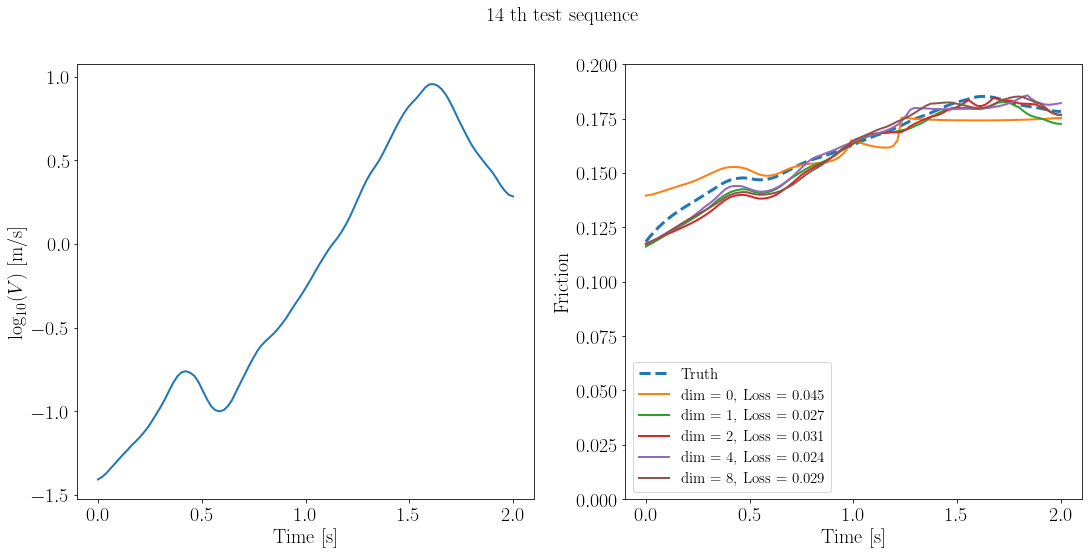
\includegraphics[width=0.9\textwidth]{images/dtTSqBurigede1.png}
    % \caption{Example sequence 1}
    \label{fig:dtTSqBurigede1}
\end{figure}

\begin{figure}[H]
    \centering
    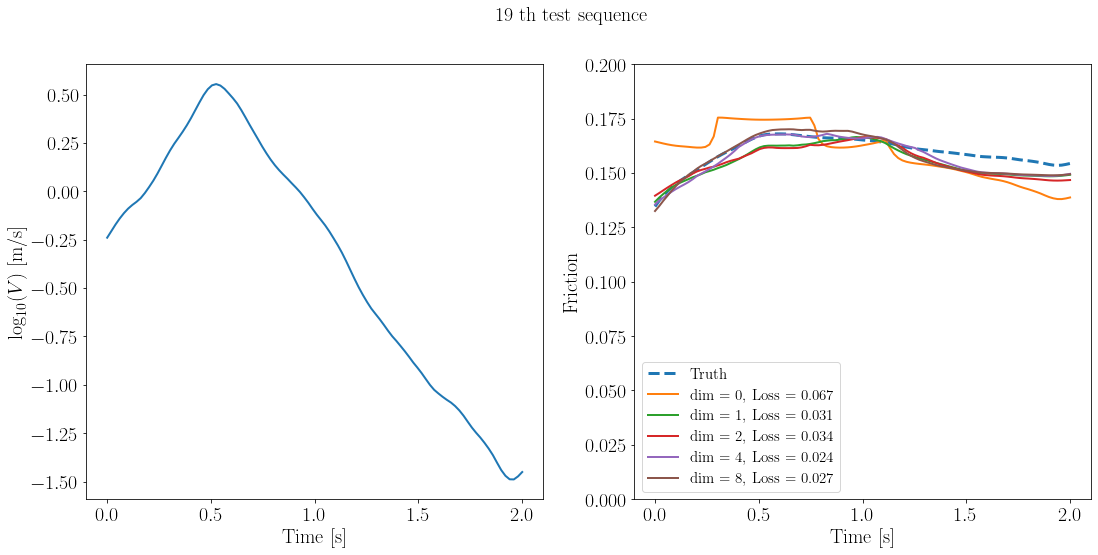
\includegraphics[width=0.9\textwidth]{images/dtTSqBurigede2.png}
    % \caption{Example sequence 2}
    \label{fig:dtTSqBurigede2}
\end{figure}
\subsubsection{Dataset with velocity-jumping sequences}
\begin{table}[H]
    \centering
    \begin{tabular}{c|ccccc}
        \hline
        dim($\xi$) & 0 & 1 & 2 & 4 & 8\\
        \hline \\[-1em]
        Test error ($p=2$) & 0.0967  & 0.0104 & 0.0154 & 0.0162 & 0.0194\\
        \hline
    \end{tabular}
    \caption{Average $L_2$ test error with different dimensions of hidden variable.}
    \label{tab:resDtTSqJump}
\end{table}
\begin{figure}[H]
    \centering
    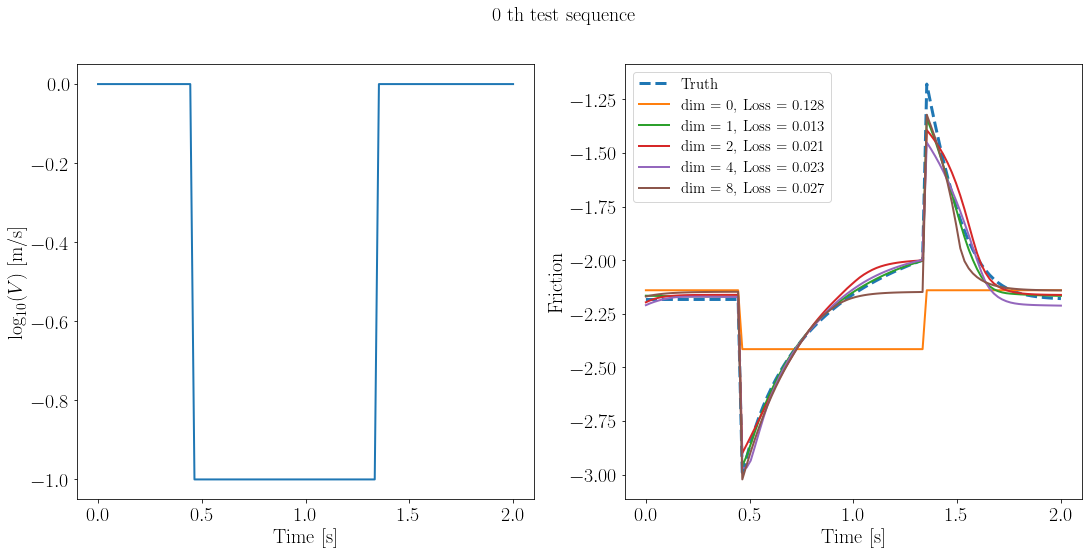
\includegraphics[width=0.9\textwidth]{images/dtTSqJump1.png}
    % \caption{Example sequence 1}
    \label{fig:dtTSqJump1}
\end{figure}

\begin{figure}[H]
    \centering
    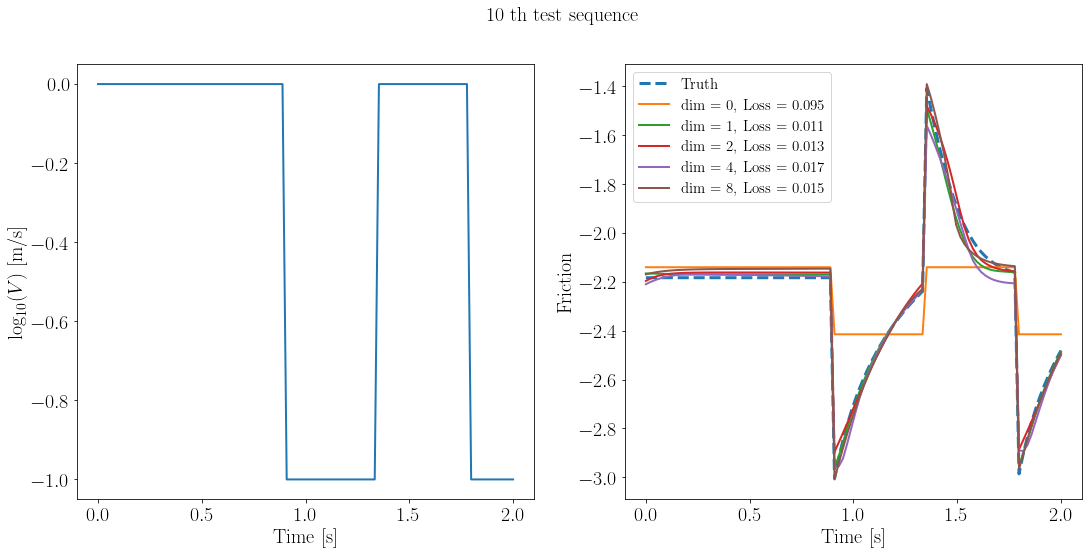
\includegraphics[width=0.9\textwidth]{images/dtTSqJump2.png}
    % \caption{Example sequence 2}
    \label{fig:dtTSqJump2}
\end{figure}

\subsection{Results with no potential formulation--optimized NN structure}
\subsubsection{Dataset of Burigede's sequences}
\begin{table}[H]
    \centering
    \begin{tabular}{c|ccccc}
        \hline
        dim($\xi$) & 0 & 1 & 2 & 4 & 8 \\
        \hline \\[-1em]
        Test error ($p=2$) & 0.0651 & 0.0399 & 0.0296 & 0.0278 & 0.0229\\
        \hline
    \end{tabular}
    \caption{Average $L_2$ test error with different dimensions of hidden variable.}
    \label{tab:resFGBurigede}
\end{table}

\begin{figure}[H]
    \centering
    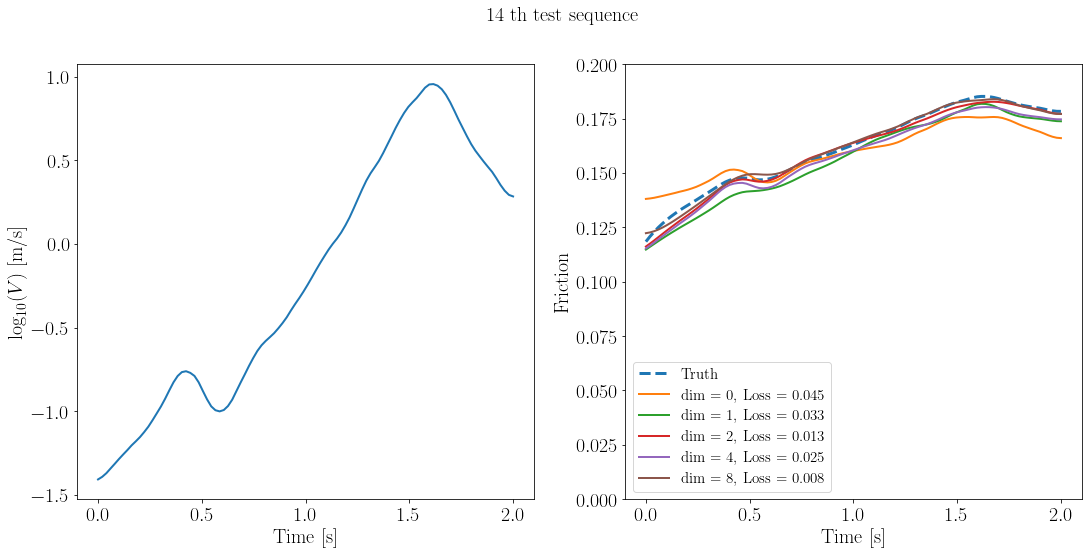
\includegraphics[width=0.9\textwidth]{images/FGBurigede1.png}
    % \caption{Example sequence 1}
    \label{fig:FGBurigede1}
\end{figure}

\begin{figure}[H]
    \centering
    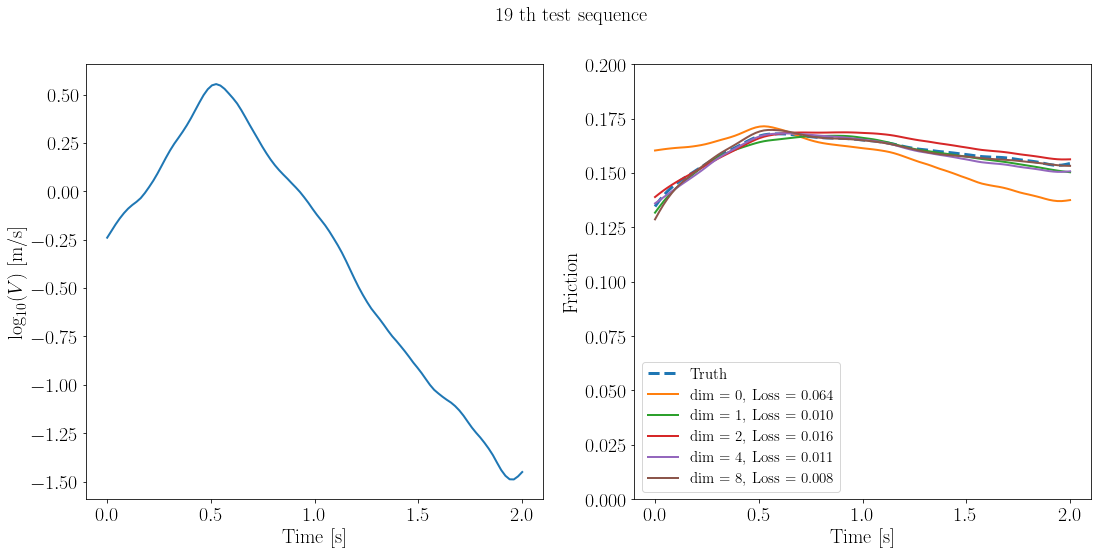
\includegraphics[width=0.9\textwidth]{images/FGBurigede2.png}
    % \caption{Example sequence 2}
    \label{fig:FGBurigede2}
\end{figure}

\subsubsection{Dataset with velocity-jumping sequences}
\begin{table}[H]
    \centering
    \begin{tabular}{c|ccccc}
        \hline
        dim($\xi$) & 0 & 1 & 2 & 4 & 8\\
        \hline \\[-1em]
        Test error ($p=2$) & 0.0967  & 0.0128 & 0.0406 & 0.0105 & 0.0139\\
        \hline
    \end{tabular}
    \caption{Average $L_2$ test error with different dimensions of hidden variable.}
    \label{tab:resFGJump}
\end{table}
\begin{figure}[H]
    \centering
    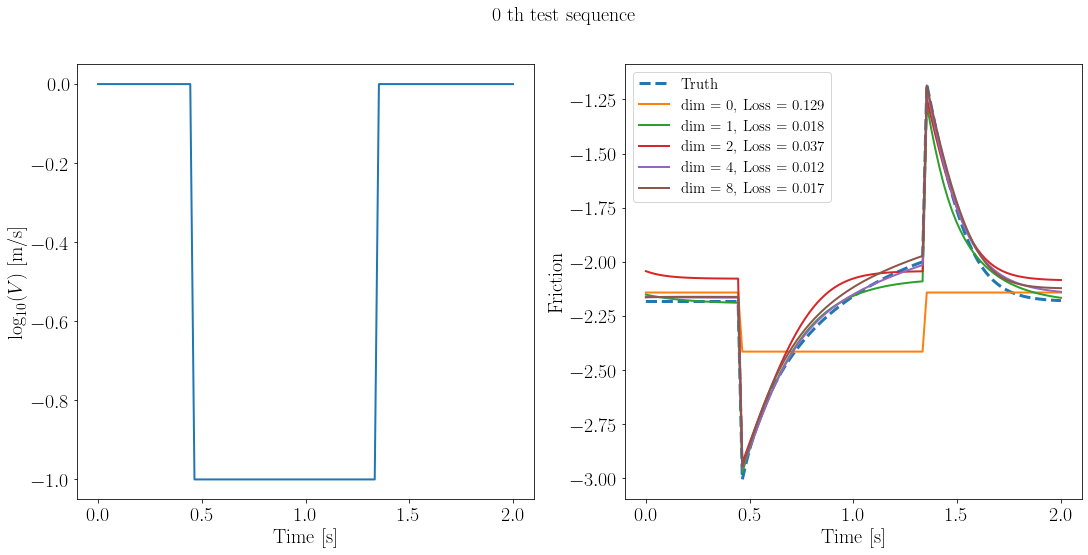
\includegraphics[width=0.9\textwidth]{images/FGJump1.png}
    % \caption{Example sequence 1}
    \label{fig:FGJump1}
\end{figure}

\begin{figure}[H]
    \centering
    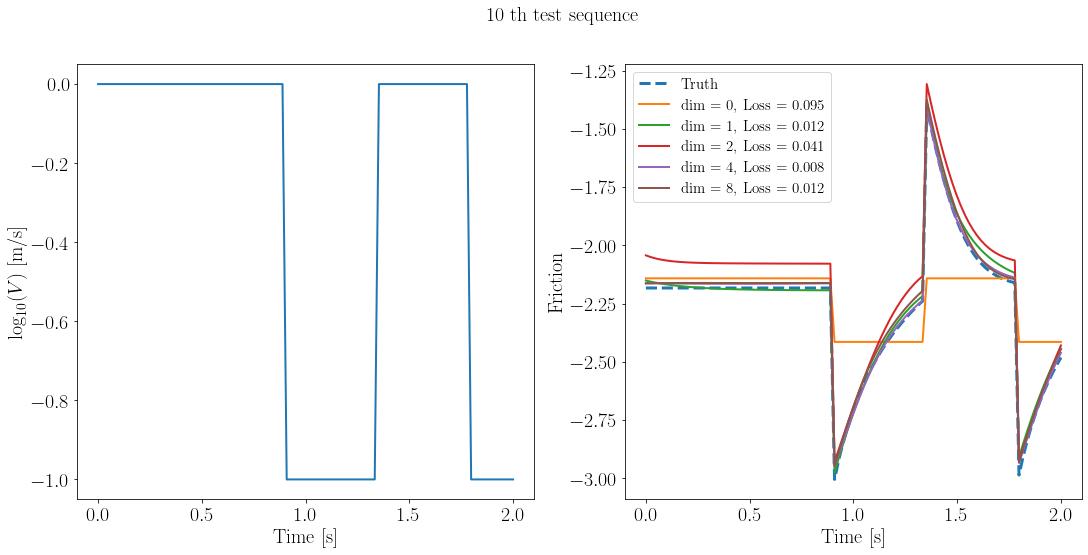
\includegraphics[width=0.9\textwidth]{images/FGJump2.png}
    % \caption{Example sequence 2}
    \label{fig:FGJump2}
\end{figure}

\newpage
\subsection{Result with the potential formulation--fixed NN structure}
\subsubsection{Dataset of Burigede's sequences}
\begin{table}[H]
    \centering
    \begin{tabular}{c|ccccc}
        \hline
        dim($\xi$) & 0 & 1 & 2 & 4 & 8 \\
        \hline \\[-1em]
        Test error ($p=2$) & 0.0660 & 0.0413 & 0.0326 & 0.0320 & 0.0288\\
        \hline
    \end{tabular}
    \caption{Average $L_2$ test error with different dimensions of hidden variable.}
    \label{tab:resDtTsqBurigedeFixed}
\end{table}

\begin{figure}[H]
    \centering
    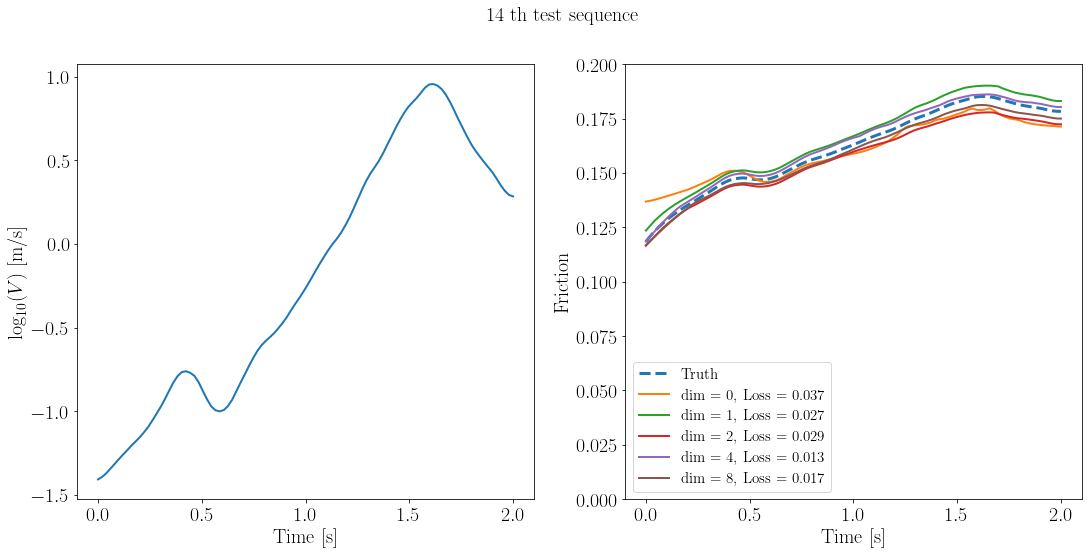
\includegraphics[width=0.9\textwidth]{images/dtTSqBurigede1_fixed.png}
    % \caption{Example sequence 1}
    \label{fig:dtTSqBurigede1Fixed}
\end{figure}

\begin{figure}[H]
    \centering
    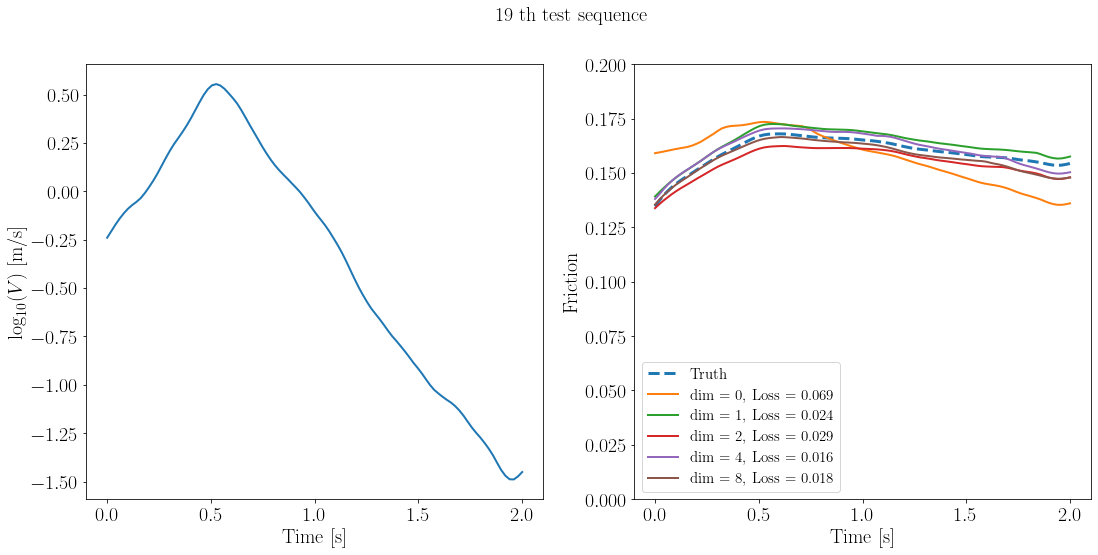
\includegraphics[width=0.9\textwidth]{images/dtTSqBurigede2_fixed.png}
    % \caption{Example sequence 2}
    \label{fig:dtTSqBurigede2Fixed}
\end{figure}
\subsubsection{Dataset with velocity-jumping sequences}
\begin{table}[H]
    \centering
    \begin{tabular}{c|ccccc}
        \hline
        dim($\xi$) & 0 & 1 & 2 & 4 & 8\\
        \hline \\[-1em]
        Test error ($p=2$) & 0.1205  & 0.0054 & 0.1020 & 0.0219 & 0.7050\\
        \hline
    \end{tabular}
    \caption{Average $L_2$ test error with different dimensions of hidden variable.}
    \label{tab:resDtTSqJumpFixed}
\end{table}
\begin{figure}[H]
    \centering
    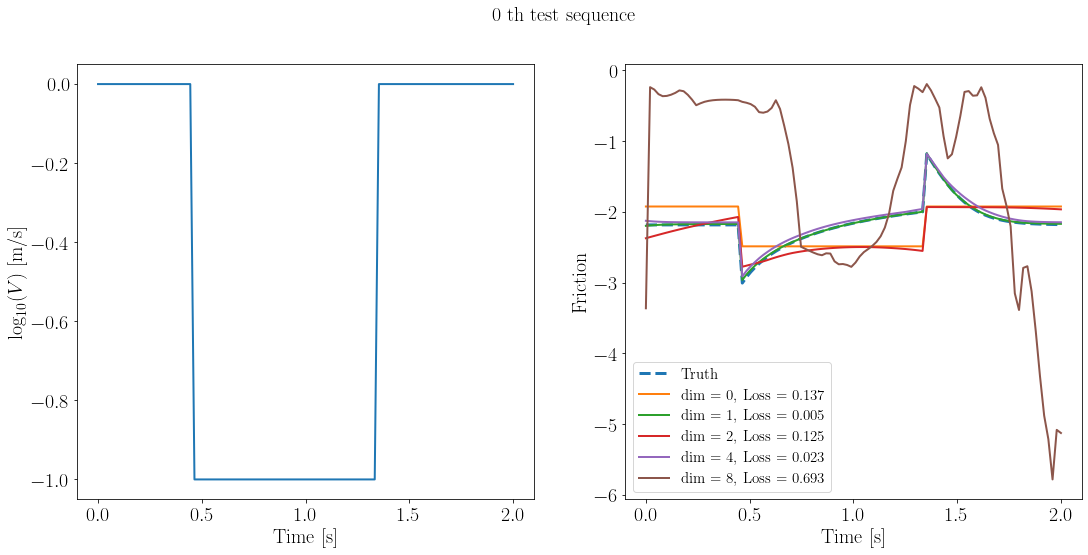
\includegraphics[width=0.9\textwidth]{images/dtTSqJump1_fixed.png}
    % \caption{Example sequence 1}
    \label{fig:dtTSqJump1Fixed}
\end{figure}

\begin{figure}[H]
    \centering
    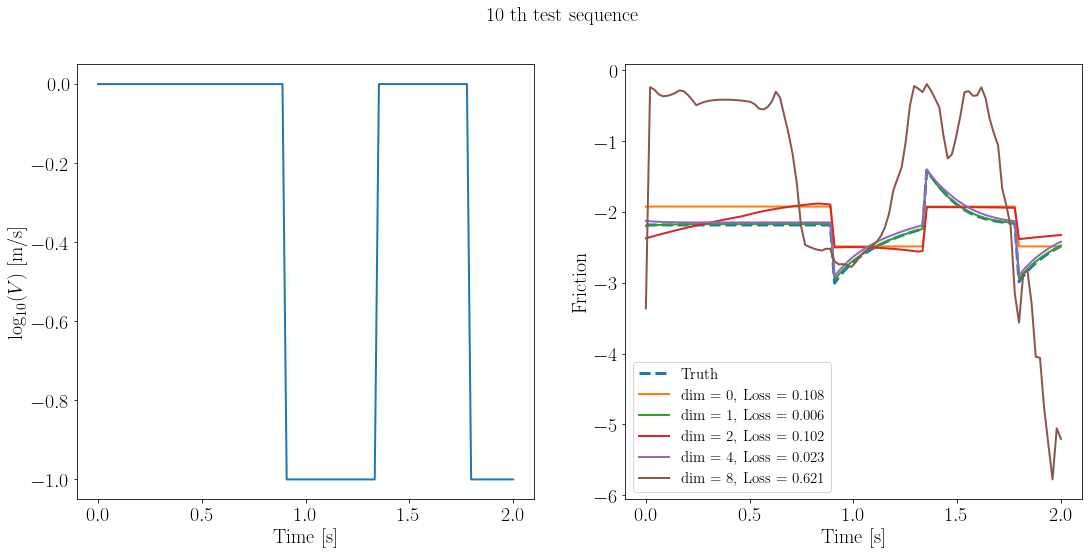
\includegraphics[width=0.9\textwidth]{images/dtTSqJump2_fixed.png}
    % \caption{Example sequence 2}
    \label{fig:dtTSqJump2Fixed}
\end{figure}

\subsection{Results with no potential formulation--fixed NN structure}
\subsubsection{Dataset of Burigede's sequences}
\begin{table}[H]
    \centering
    \begin{tabular}{c|ccccc}
        \hline
        dim($\xi$) & 0 & 1 & 2 & 4 & 8 \\
        \hline \\[-1em]
        Test error ($p=2$) & 0.0632 & 0.0239 & 0.0406 & 0.0242 & 0.0192\\
        \hline
    \end{tabular}
    \caption{Average $L_2$ test error with different dimensions of hidden variable.}
    \label{tab:resFGBurigedeFixed}
\end{table}

\begin{figure}[H]
    \centering
    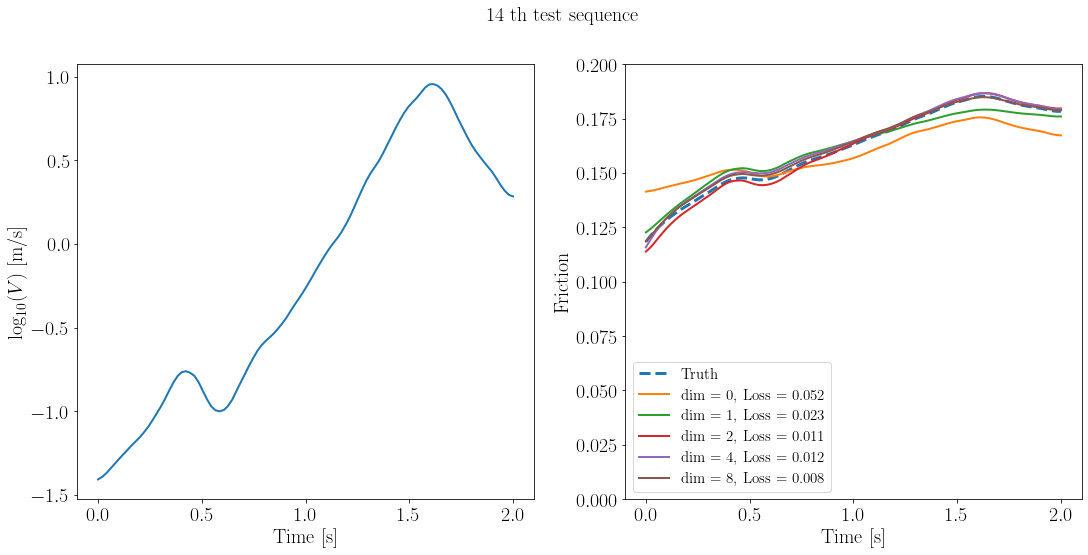
\includegraphics[width=0.9\textwidth]{images/FGBurigede1_fixed.png}
    % \caption{Example sequence 1}
    \label{fig:FGBurigede1Fixed}
\end{figure}

\begin{figure}[H]
    \centering
    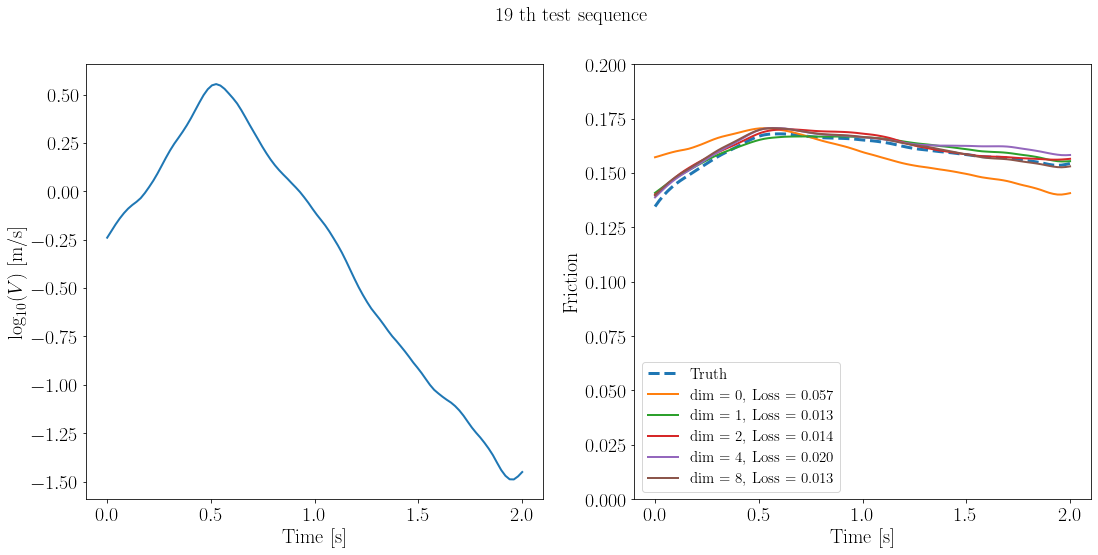
\includegraphics[width=0.9\textwidth]{images/FGBurigede2_fixed.png}
    % \caption{Example sequence 2}
    \label{fig:FGBurigede2Fixed}
\end{figure}

\subsubsection{Dataset with velocity-jumping sequences}
\begin{table}[H]
    \centering
    \begin{tabular}{c|ccccc}
        \hline
        dim($\xi$) & 0 & 1 & 2 & 4 & 8\\
        \hline \\[-1em]
        Test error ($p=2$) & 0.01286  & 0.0117 & 0.0119 & 0.0163 & 0.0072\\
        \hline
    \end{tabular}
    \caption{Average $L_2$ test error with different dimensions of hidden variable.}
    \label{tab:resFGJumpFixed}
\end{table}
\begin{figure}[H]
    \centering
    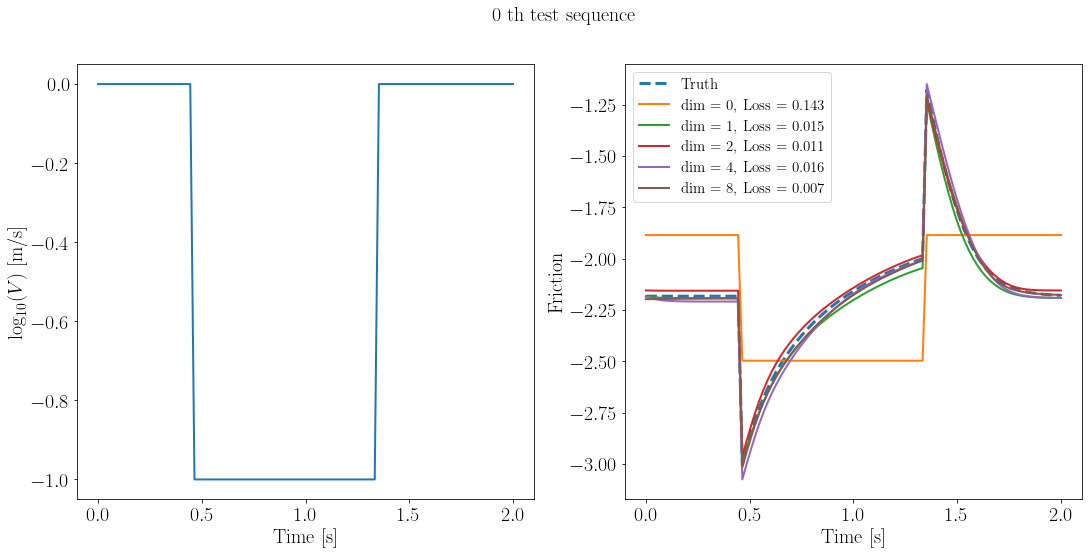
\includegraphics[width=0.9\textwidth]{images/FGJump1_fixed.png}
    % \caption{Example sequence 1}
    \label{fig:FGJump1Fixed}
\end{figure}

\begin{figure}[H]
    \centering
    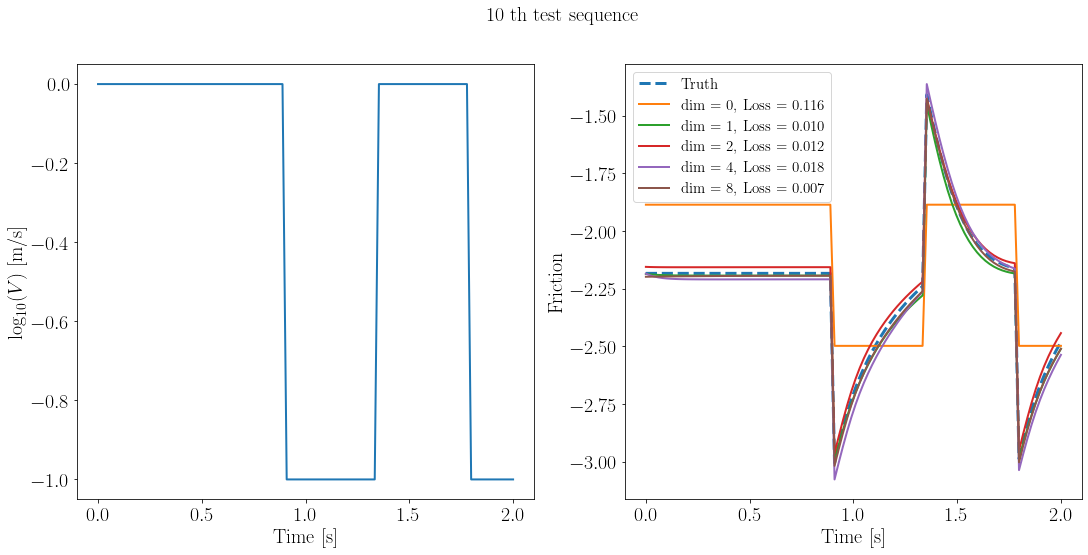
\includegraphics[width=0.9\textwidth]{images/FGJump2_fixed.png}
    % \caption{Example sequence 2}
    \label{fig:FGJump2Fixed}
\end{figure}

\section{Training and testing on different generated datasets}
Here we use two different methods to generate the training dataset (one being Burigede's continuous variations, one being velocity-jump tests), 
with the same friction parameters:
\begin{align*}
    a = 0.011, b = 0.016, D_{RS} = 0.1\ \mathrm{m}, f_* = 0.58.
\end{align*}

Since the fluctuations of friction around the steady-state friction coefficient $f_{ss} $will be of the same order as $a$, 
and $a$ is of $1$ to $2$ orders of magnetitudes smaller than $f_{ss}$, 
a re-scaling scheme is needed for better training performance. 
Here we transform the training $f_{targ}$'s through the following re-scaling scheme:
\begin{align}
    \hat{f}_{targ}(t) = \mathcal{T}\left[{f}_{targ}(t)\right] = \alpha_{scaling}  \left({f}_{targ}(t) - f_{offset}\right) + f_{offset}, \label{eq:rescalingScheme}
\end{align}
where $\alpha_{scaling}$ is a scaling factor (here I used 50), 
$f_{offset}$ is the offset constant (I used $0.52$). 

Then the model is trained on the relative $L_2$ loss between $\hat{f}_{pred}(t)$ and $\hat{f}_{targ}(t)$, 
and finally we re-scale $\hat{f}_{pred}(t)$ back to get $f_{pred}(t)$, i.e., 
\begin{align*}
    {f}_{pred}(t) = \mathcal{T}^{-1}\left[\hat{f}_{pred}(t)\right]. 
\end{align*}

Below I first show some fits of $2$ trained models on their corresponding datasets, 
and then I show the results of the cross-performance of the $2$ models on the other dataset that they were not trained on, (for example, the fits on the velocity-jump dataset of the model trained on Burigede's dataset). 

\noindent \textbf{What I have observed is that}, 
\begin{itemize}
    \item Each model can fit to the dataset they were trained on fairly well, 
    but the performance is bad on the dataset they have not been trained on.
    \item It is easier to fit the velocity-jump dataset than Burigede's dataset. 
\end{itemize}

\newpage
\subsection{Model performances on the dataset they were trained on}
\subsubsection{Velocity-jump dataset}
\begin{figure}[H]
    \centering
    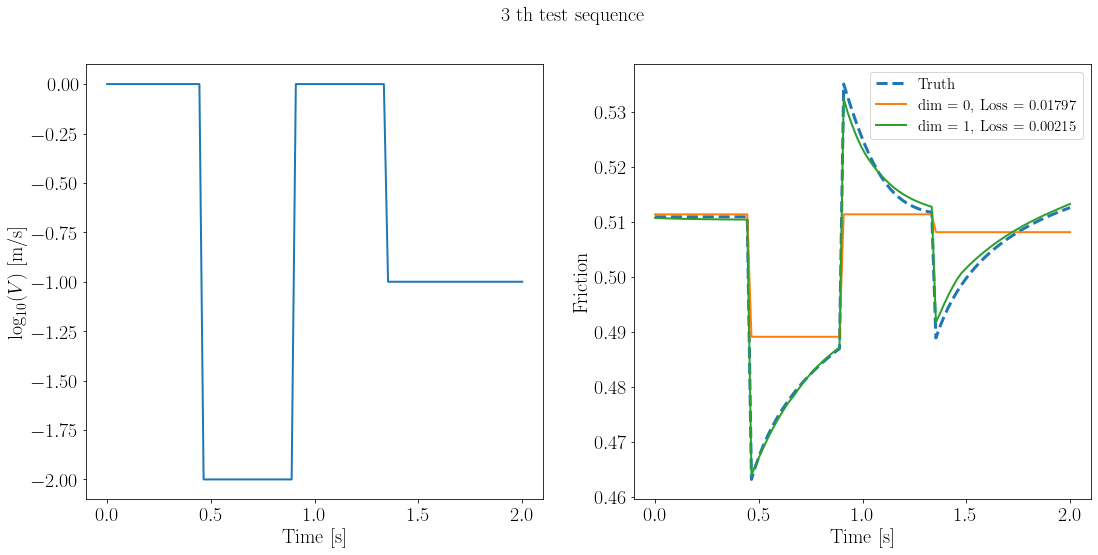
\includegraphics[width=0.9\textwidth]{images/dtTSqJump1204_1.png}
    % \caption{Example sequence 1}
    \label{fig:dtTSqJump1204_1}
\end{figure}

\begin{figure}[H]
    \centering
    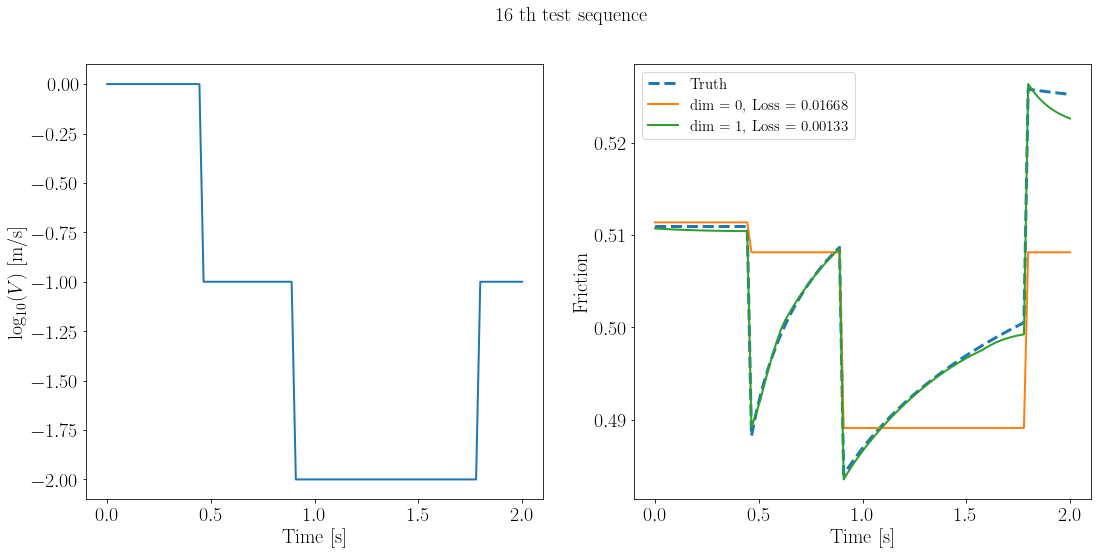
\includegraphics[width=0.9\textwidth]{images/dtTSqJump1204_2.png}
    % \caption{Example sequence 1}
    \label{fig:dtTSqJump1204_2}
\end{figure}

\subsubsection{Burigede's dataset}
\begin{figure}[H]
    \centering
    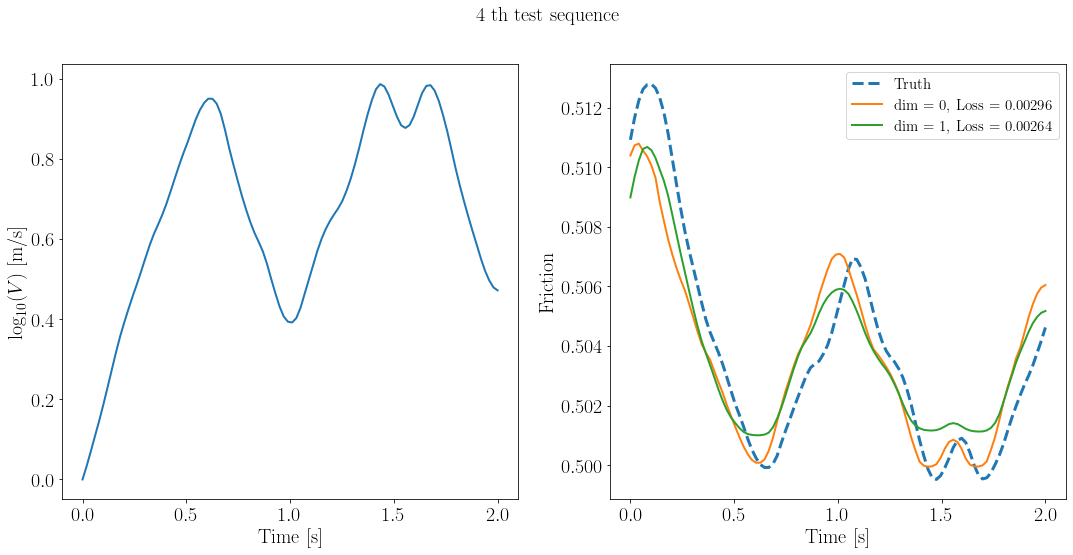
\includegraphics[width=0.9\textwidth]{images/dtTSqBurigede1204_1.png}
    % \caption{Example sequence 1}
    \label{fig:dtTSqBurigede1204_1}
\end{figure}

\begin{figure}[H]
    \centering
    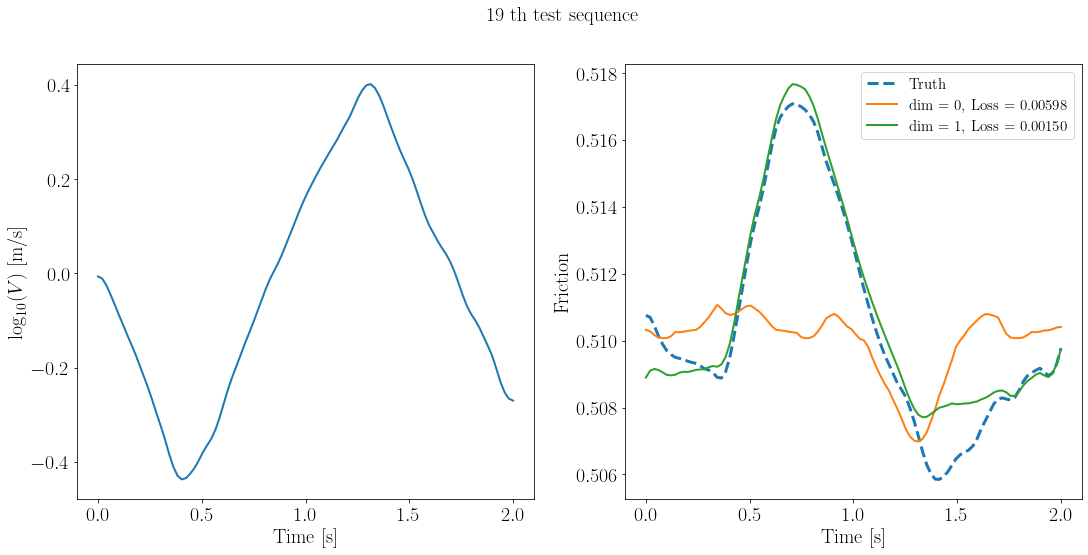
\includegraphics[width=0.9\textwidth]{images/dtTSqBurigede1204_2.png}
    % \caption{Example sequence 1}
    \label{fig:dtTSqburigede1204_2}
\end{figure}

\subsection{Model performances on the dataset they were Not trained on}
\subsubsection{Trained on Velocity-jump dataset, 
fitting performance on Burigede's dataset}
\begin{figure}[H]
    \centering
    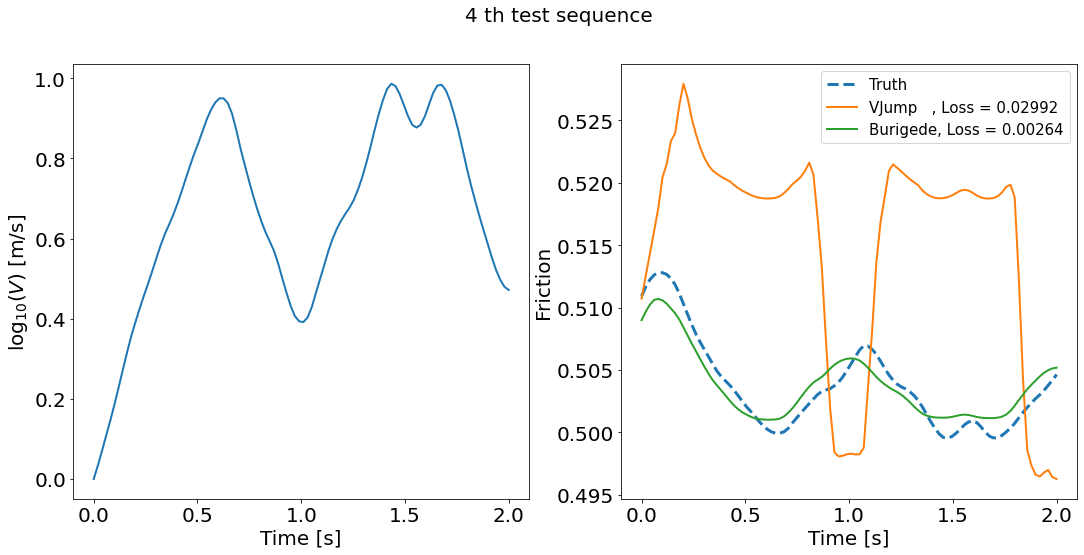
\includegraphics[width=0.9\textwidth]{images/dtTSqJumpBurigede1204_1.png}
    % \caption{Example sequence 1}
    \label{fig:dtTSqJumpBurigede1204_1}
\end{figure}

\begin{figure}[H]
    \centering
    \includegraphics[width=0.9\textwidth]{images/dtTSqJumpBurigede1204_2.png}
    % \caption{Example sequence 1}
    \label{fig:dtTSqJumpBurigede1204_2}
\end{figure}

\subsubsection{Trained on Burigede's dataset, 
fitting performance on velocity-jump dataset}
\begin{figure}[H]
    \centering
    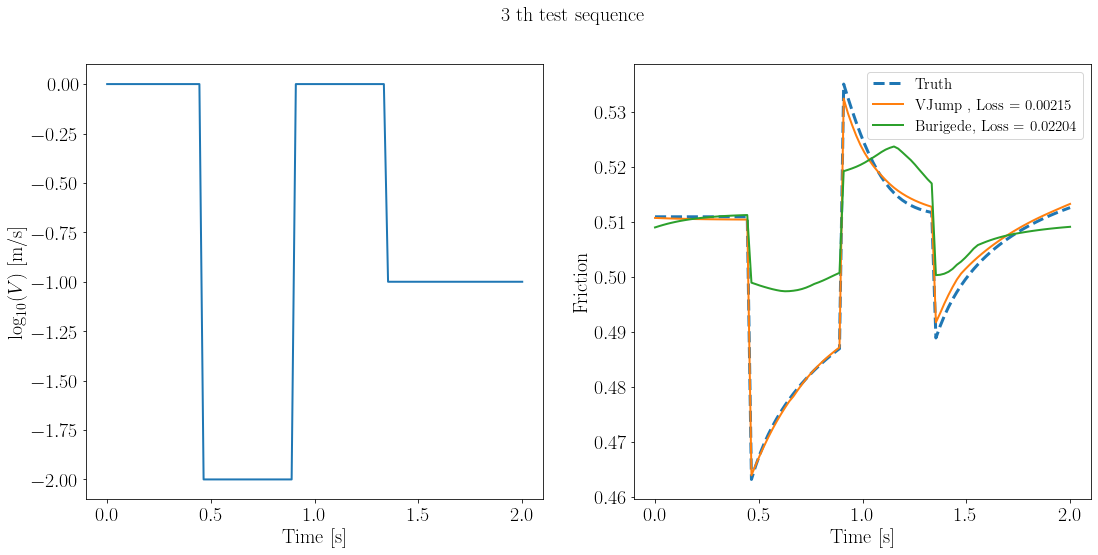
\includegraphics[width=0.9\textwidth]{images/dtTSqBurigedeJump1204_1.png}
    % \caption{Example sequence 1}
    \label{fig:dtTSqBurigedeJump1204_1}
\end{figure}

\begin{figure}[H]
    \centering
    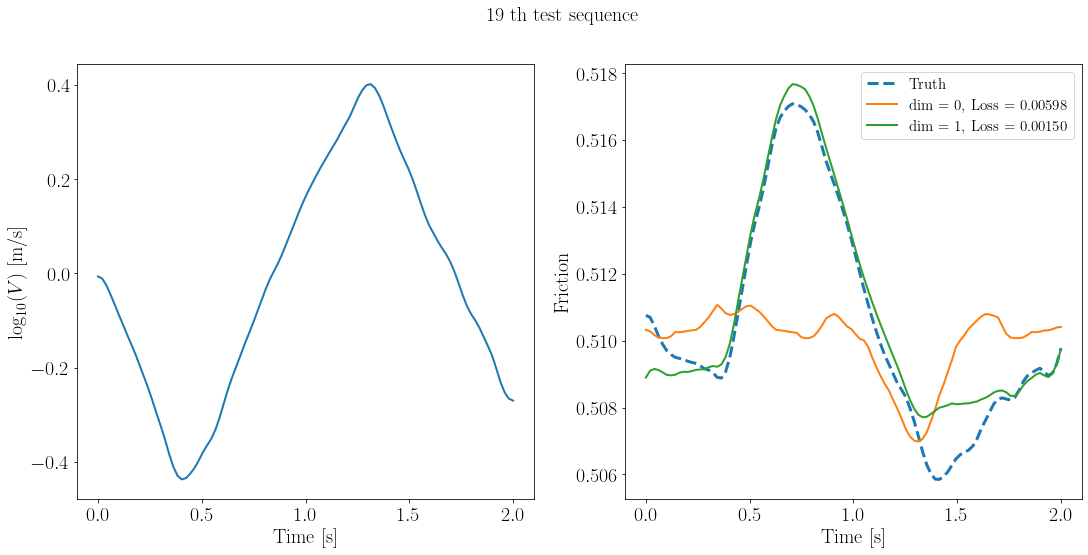
\includegraphics[width=0.9\textwidth]{images/dtTSqBurigede1204_2.png}
    % \caption{Example sequence 1}
    \label{fig:dtTSqBurigedeJump1204_2}
\end{figure}

\begin{comment}
\begin{table}[H]
    \centering
    \begin{tabular}{c|cccc}
        \hline
        dim($\xi$) & 0 & 1 & 2 & 4 \\
        \hline \\[-1em]
        Test error ($p=2$) & 0.20652& 0.20353 & 0.20352 & 0.20352\\
        \hline
    \end{tabular}
    \caption{Average $L_2$ test error with different dimensions of hidden variable $\bm{\xi}$ with $D(\dot{\xi})=\frac{1}{2}|\dot{\xi}|^2$.}
    \label{tab:resSimpleXi}
\end{table}

\subsection{Set $D(\dot{\xi}) = \frac{1}{2}\dot{\xi}^2  + D^{exp}(\dot{\xi})$}
Here we allow $D(\dot{\bm{\xi}})$ to have a correction term 
$D^{exp} (\dot{\bm{\xi}})$, 
which is treated explicitly in the update of $\bm{\xi}$. 
Then equation (\ref{eq:redEqn1}) would have an additional correction term as 
\begin{align}
    \dot{\bm{\xi}} &= \frac{\bm{\xi}_{n+1} - \bm{\xi}_n}{t_{n+1}-t_{n}} = -\frac{\partial {W}}{\partial \bm{\xi}}(\dot{x}_n, \bm{\xi}_n) - 
    \frac{\partial D^{exp}}{\partial \dot{\bm{\xi}}}(\dot{\bm{\xi}}_n),  \label{eq:redEqn2}
\end{align}
where $W(\dot{x}, \bm{\xi}_n), D^{exp}(\dot{\bm{\xi}})$ are approximated by Neural Networks, 
and $\dot{\bm{\xi}}_n$ is calculated explicitly from previous time-steps as 
\begin{align*}
    \dot{\bm{\xi}}_n = \frac{\bm{\xi}_n-\bm{\xi}_{n-1}}{t_n - t_{n-1}}.
\end{align*}

\begin{table}[H]
    \centering
    \begin{tabular}{c|cccc}
        \hline
        dim($\xi$) & 0 & 1 & 2 & 4 \\
        \hline \\[-1em]
        Test error ($p=2$) & 0.20652& 0.20998 & 0.20997 & 0.20997\\
        \hline
    \end{tabular}
    \caption{Average $L_2$ test error with different dimensions of hidden variable $\bm{\xi}$ with $D(\dot{\xi})=\frac{1}{2}|\dot{\xi}|^2+D^{exp}(\dot{\xi})$.}
    \label{tab:resSimpleXi}
\end{table}

\subsection{Learning the Legendre transform of $D(\dot{\xi})$}
\noindent Suppose $D(\dot{\bm{\xi}}) : \mathbb{R}^d \rightarrow \mathbb{R}$ is convex in $\bm{\dot{\xi}}$, 
then the Legendre transform of $D$, 
\begin{align*}
    D^*\left(\dot{\bm{d}}\right) &= \sup_{\dot{\bm{\xi}} \in \mathbb{R}^d} \left\{\la \dot{\bm{d}}, \dot{\bm{\xi}}\ra - D\left(\dot{\bm{\xi}}\right)\right\}
\end{align*}
satisifies 
\begin{align}
    \frac{\partial D^*}{\partial \dot{\bm{d}}} \left(\frac{\partial D}{\partial \dot{\bm{\xi}}}\left(\dot{\bm{\xi}}\right)\right) &= \dot{\bm{\xi}}. \label{eq:LegKey}
\end{align}
Then the red equation can be solved by
\begin{align}
    \dot{\bm{\xi}} &=\frac{\bm{\xi}_{n+1} - \bm{\xi}_n}{t_{n+1}-t_{n}} = \frac{\partial D^*}{\partial \dot{\bm{d}}} \left(-\frac{\partial W}{\partial {\bm{\xi}}}\left({\bm{\xi}}\right)\right),  \label{eq:redEqn2}
\end{align}
where $D^*$ is the only function that requires $NN$ approximation. 

\begin{figure}[H]
    \centering
    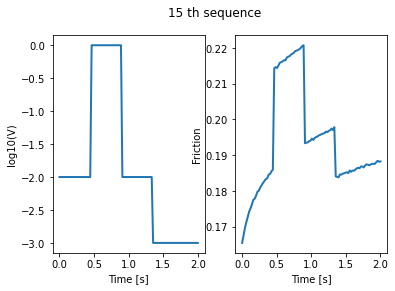
\includegraphics[width=0.6\textwidth]{images/exampleSeq1.png}
    \caption{Example sequence 1}
    \label{fig:ExSeq1}
\end{figure}
\begin{figure}[H]
    \centering
    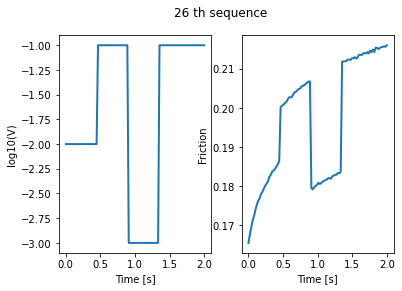
\includegraphics[width=0.6\textwidth]{images/exampleSeq2.png}
    \caption{Example sequence 2}
    \label{fig:ExSeq2}
\end{figure}
\noindent Figure~\ref{fig:ExSeq1} and \ref{fig:ExSeq2} shows two examples of the generated sequence used for training and testing. 

\noindent Below are two tables showing the result given by setting the potentials to $\{W(\dot{x}, \bm{\xi}), D(\dot{\bm{\xi}})\}$ \textbf{or} $\{W(x, \bm{\xi}), D^\dagger(\dot{x}), D(\dot{\bm{\xi}})\}$, setting activation function to $ELU$, respectively, 
and with Legendre transform. 

\begin{table}[H]
    \centering
    \begin{tabular}{c|ccccc}
        \hline
        dim($\xi$) & 0 & 1 & 2 & 4 & 8\\
        \hline \\[-1em]
        Test error ($p=2$) & 0.05075& 0.02790 & 0.03180 & 0.02825 & 0.02910\\
        \hline
    \end{tabular}
    \caption{Average $L_2$ test error with different dimensions of hidden variable $\bm{\xi}$ with learning $\{W(\dot{x}, \bm{\xi}), D(\dot{\bm{\xi}})\}$ as shown in (\ref{eq:nToNPlusOneDotX}), and activation function $ELU$.}
    \label{tab:legELUWD}
\end{table}

\begin{table}[H]
    \centering
    \begin{tabular}{c|ccccc}
        \hline
        dim($\xi$) & 0 & 1 & 2 & 4 & 8\\
        \hline \\[-1em]
        Test error ($p=2$) & 0.05146& 0.02404 & 0.02275 & 0.02338 & 0.02532\\
        \hline
    \end{tabular}
    \caption{Average $L_2$ test error with different dimensions of hidden variable $\bm{\xi}$ with learning $\{W(x, \bm{\xi}), D^\dagger(\dot{x}), D(\dot{\bm{\xi}})\}$ as shown in (\ref{eq:nToNPlusOneDotXDagger}), and activation function $ELU$.}
    \label{tab:legELUWDDDagger}
\end{table}
\end{comment}

\begin{comment}
\noindent I think it makes sense to set $W = W(\dot{x}, \bm{\xi})$ instead of $W(x, \bm{\xi})$, 
since 
\begin{itemize}
    \item Due to material frame indifference, $F_{fric}$ should largely not depend on displacement $x$, 
    (it can depend on $x$ via the hidden variables $\xi$, but not strong enough to show up in $W$ explicitly.) 
    \item As we can see from (\ref{eq:nToNPlusOneDotX}), 
    having $W(\dot{x}, \bm{\xi}), D^*(\dot{\bm{d}})$ still allows for an optimization formulation for solving the ODE system, 
    which is our goal. 
    \item The results show that $W(\dot{x}, \bm{\xi})$ has much better accuracy than $W(x, \bm{\xi})$, 
    which makes sense because for small slip rates, 
    $x$ is always almost $0$, 
    while for $\dot{x}$ if we pass in $\log(\dot{x})$, 
    the precision will be much higher. 
\end{itemize}
\end{comment}
\begin{comment}
\subsection{Learning in a boosted manner}
We observed that the rate-dependence usually dominates in rate-and-state friction and then we should learn this in a boosted manner. 
For the first round, 
we only learn the rate effect, i.e., 
we only try to fit
\begin{align}
    f_0 &= \frac{\partial W_0}{\partial x}(x) + \frac{\partial D^\dagger}{ \partial \dot{x}}(\dot{x}), \label{eq:boostingBase}
\end{align}
by training two NNs for $W_0(x)$ and $D^\dagger(\dot{x})$ minimizing $Loss(f_0(x, \dot{x}), f_{targ})$. 
Then we can fit
\begin{align}
    f_1 = \frac{\partial W_1}{\partial x}(x, \bm{\xi}) \label{eq:boostingXi}\\ 
    \frac{\partial{W_1}}{\partial \bm{\xi}} (x, \bm{\xi}) + \frac{\partial D}{\partial \dot{\bm{\xi}}} = 0. \label{eq:boostingEvolution}
\end{align}
to the residual of $f_targ - f_0$ by training  additional two NNs $W_1(x, \bm{\xi})$ and $D^*(d\dot{\bm{d}})$ (the Legendre transform of $D(\bm{\xi})$). 
This round $Loss(f_1, f_{targ} - f_0)$ is minimized. 
Then we have our final estimate as 
\begin{align}
    f(t) &= f_0(t) + f_1(t). \label{eq:boostingFinalEstimate}
\end{align}

Another issue we encountered is that since rate-and-state friction $f(t)$'s have only small variations around a reference value, say $f_{ref} = 0.5$, 
the normalization in the loss function needs to be modified to 
\begin{align}
    Loss(f_{targ}, f; p, f_{ref}) = \frac{1}{|I|} \sum_{i\in I} \frac{\|f(t)-f_{targ}(t)\|_p}{\|f_{targ}(t) - f_{ref}\|_p} \label{eq:offsetLoss}. 
\end{align}
It is important to note that the modified loss function \textbf{would not fundamentally affect the training process}, 
since we are essentially changing the weight of the error of each sequence in the total error.

\subsubsection{Burigede's generation method with large $D_{RS}$}
These are results from a dataset generated using Burigede's data-generation manner and with large $D_{RS}$ such that the friction is never at steady-state.

\begin{table}[H]
    \centering
    \begin{tabular}{c|ccc}
        \hline
        dim($\xi$) & 0 & 1 & 2\\
        \hline \\[-1em]
        Test error ($p=2$) & 0.0730& 0.0318 & 0.0314\\
        \hline
    \end{tabular}
    \caption{Average $L_2$ test error with different dimensions of hidden variable $\bm{\xi}$ with learning $\{W(\dot{x}, \bm{\xi}), D(\dot{x}), D(\dot{\bm{\xi}})\}$ in a \textbf{boosted manner}, as shown in (\ref{eq:nToNPlusOneDotX}), and activation function $ELU$.}
    \label{tab:legELUWDBoosted}
\end{table}

A \textbf{representative example} of fit in the test dataset :
\begin{figure}[H]
    \centering
    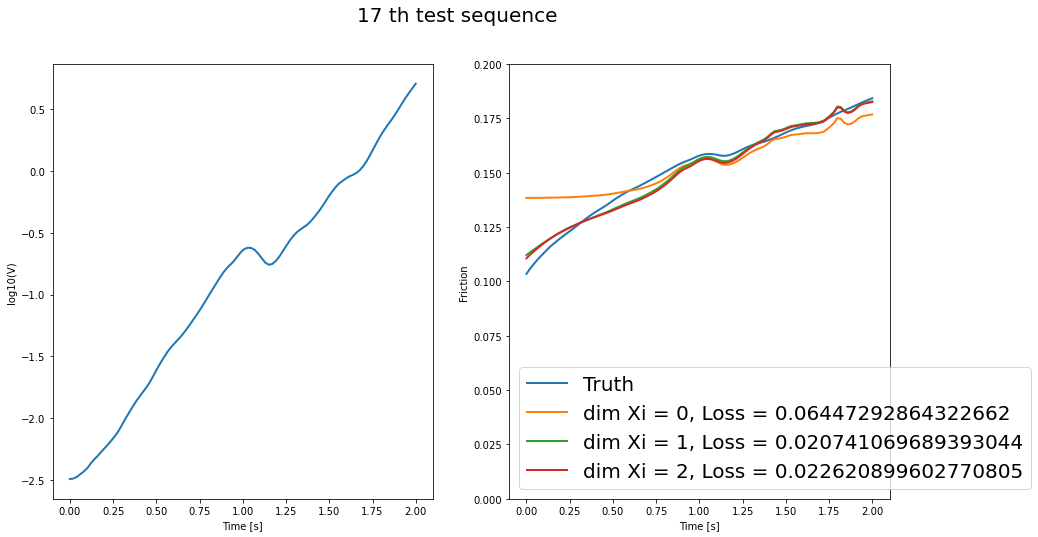
\includegraphics[width=0.8\textwidth]{images/boosted_algorithm_seq1.png}
    \caption{Example sequence 1 with fixed scaling of $0 \le y \le 0.2$. }
    \label{fig:BoostedSeq1}
\end{figure}
\begin{figure}[H]
    \centering
    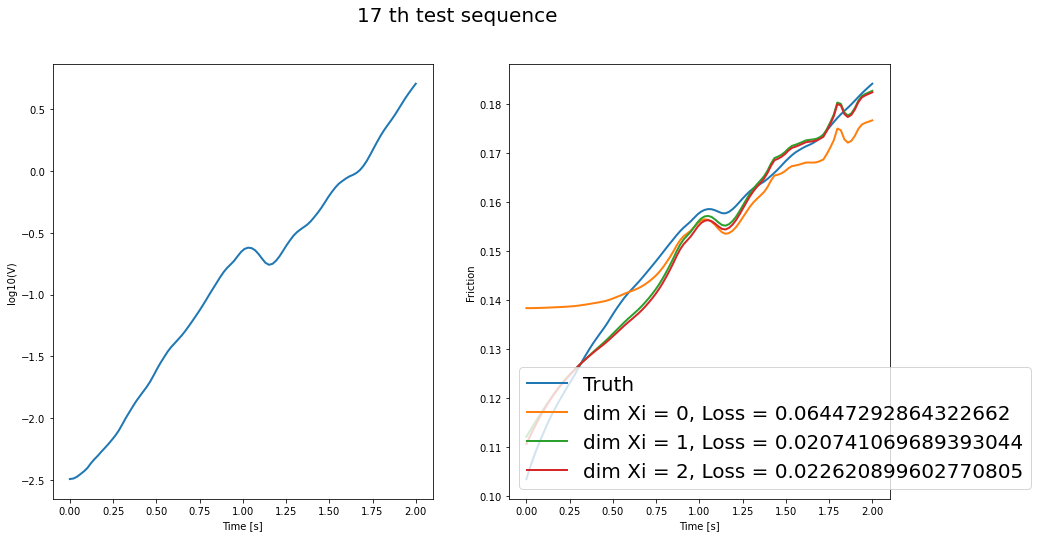
\includegraphics[width=0.8\textwidth]{images/boosted_algorithm_seq1_noFixedScaling.png}
    \caption{Example sequence 1 with unfixed scaling. }
    \label{fig:BoostedSeq1UnFixedScaling}
\end{figure}

A \textbf{bad-extreme} example of fit in the test dataset :
\begin{figure}[H]
    \centering
    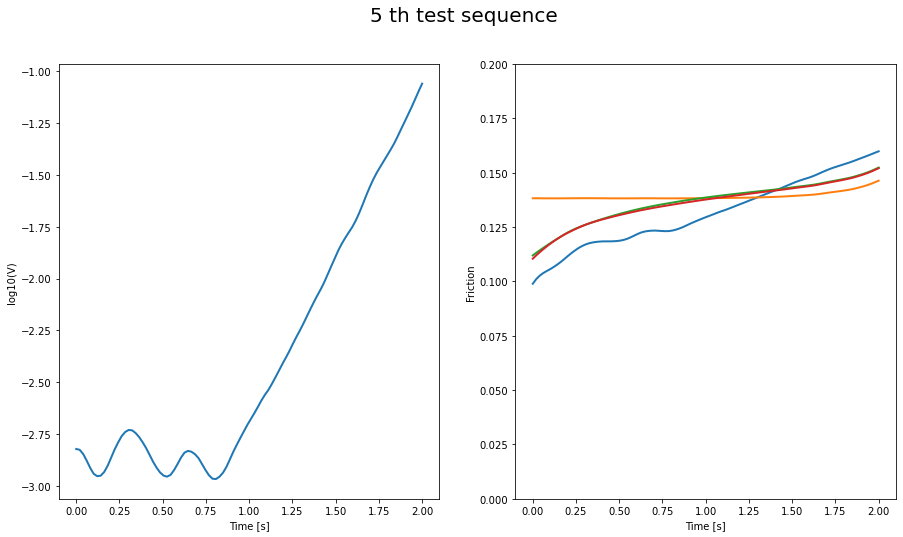
\includegraphics[width=0.8\textwidth]{images/boosted_algorithm_seq2.png}
    \caption{Example sequence 2 with fixed scaling of $0 \le y \le 0.2$. }
    \label{fig:BoostedSeq2}
\end{figure}
\begin{figure}[H]
    \centering
    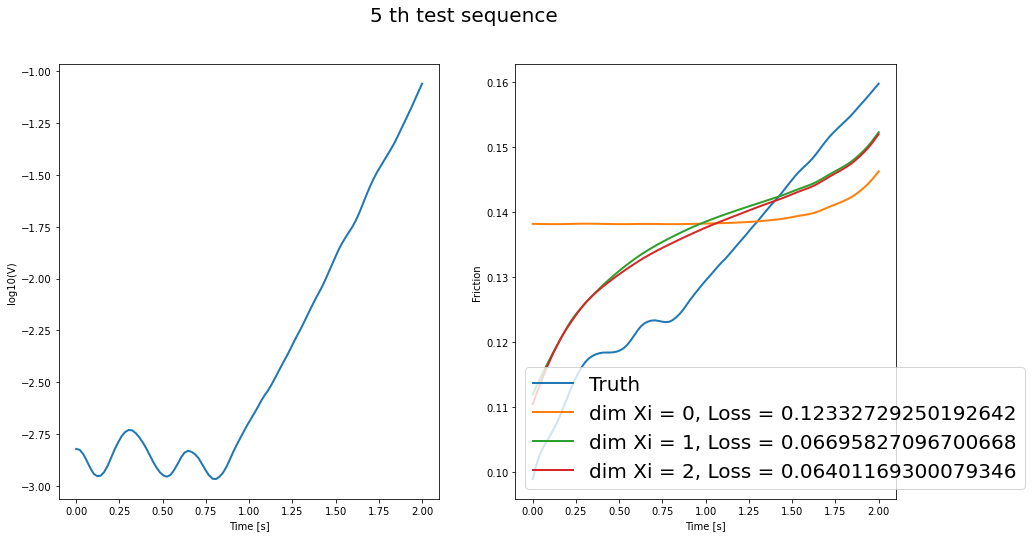
\includegraphics[width=0.8\textwidth]{images/boosted_algorithm_seq2_noFixedScaling.png}
    \caption{Example sequence 2 with unfixed scaling. }
    \label{fig:BoostedSeq2UnFixedScaling}
\end{figure}

\subsubsection{The model cannot learn jump-tests well} 
Here are some sequences of velocity-jump tests. I have adjusted the parameters to make the fluctuations in friction upon rate changes comparable to its reference value $f_{ref}$ so no need to adjust the loss function. 
But the fits look bad. 

\begin{table}[H]
    \centering
    \begin{tabular}{c|cccc}
        \hline
        dim($\xi$) & 0 & 1 & 4 & 16\\
        \hline \\[-1em]
        Test error ($p=2$) & 0.0967 & 0.0967 & 0.0967 & 0.0980\\
        \hline
    \end{tabular}
    \caption{Average $L_2$ test error on velocity-jump dataset, with different dimensions of hidden variable $\bm{\xi}$ with learning $\{W(\dot{x}, \bm{\xi}), D(\dot{x}), D(\dot{\bm{\xi}})\}$ in a \textbf{boosted manner}, as shown in (\ref{eq:boostingFinalEstimate}), and activation function $ELU$.}
    \label{tab:legELUWDBoostedVjump}
\end{table}

\begin{figure}[H]
    \centering
    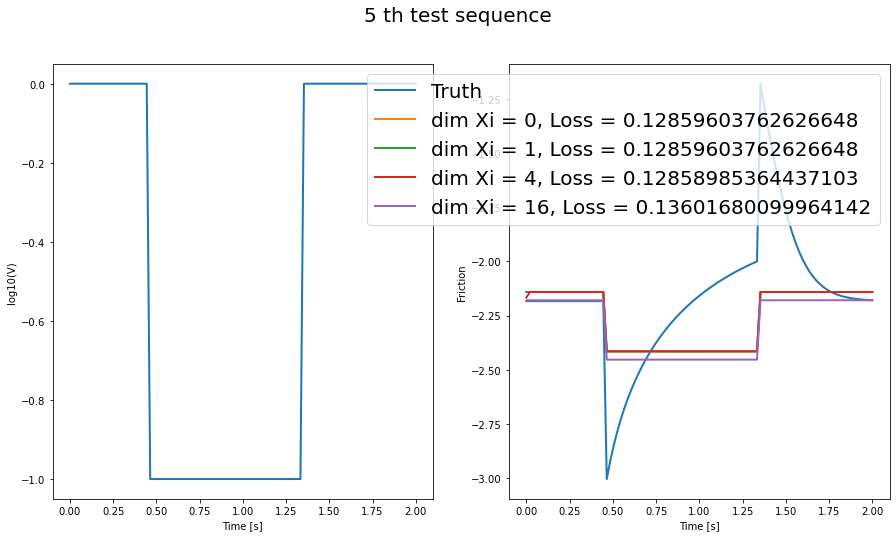
\includegraphics[width=0.8\textwidth]{images/boosted_algorithm_Vjump_seq1_noFixedScaling.png}
    \caption{Example sequence 1. }
    \label{fig:BoostedSeq1VJump}
\end{figure}
\begin{figure}[H]
    \centering
    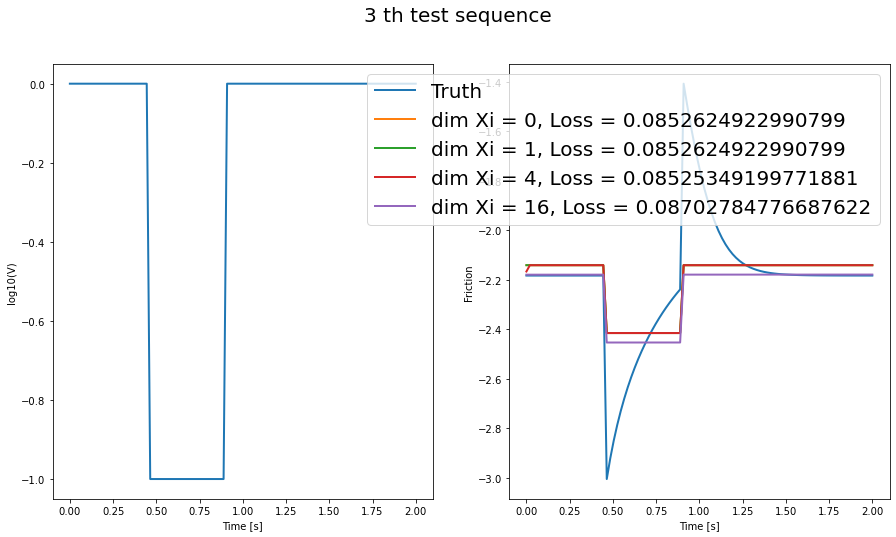
\includegraphics[width=0.8\textwidth]{images/boosted_algorithm_Vjump_seq2_noFixedScaling.png}
    \caption{Example sequence 2. }
    \label{fig:BoostedSeq2VJump}
\end{figure}
\begin{figure}[H]
    \centering
    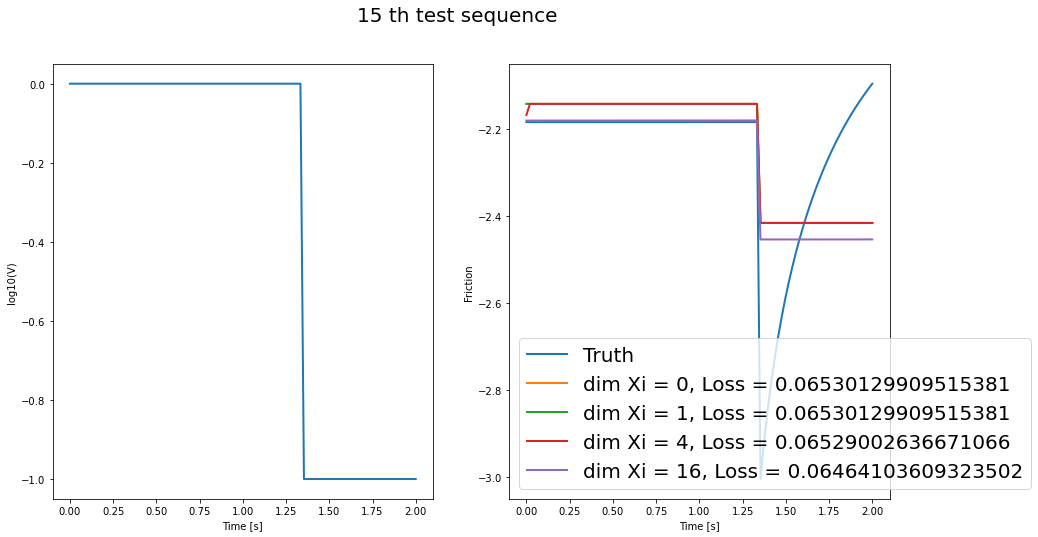
\includegraphics[width=0.8\textwidth]{images/boosted_algorithm_Vjump_seq3_noFixedScaling.png}
    \caption{Example sequence 3. }
    \label{fig:BoostedSeq3VJump}
\end{figure}
\end{comment}
\end{document}
